\documentclass[italian,a4paper,twosides,headinclude]{scrbook}
\usepackage{amsmath,amssymb,amsthm,thmtools}
\usepackage{mathtools} % per \MoveEqLeft
\usepackage{babel,a4}
\usepackage[nochapters,pdfspacing]{classicthesis}
\usepackage[utf8]{inputenc}
\usepackage{comment} % for the comment environment
\usepackage{graphicx}
\usepackage{tikz}
\usepackage{pst-node}
\usetikzlibrary{cd} % commutative diagrams
\usepackage{eucal}
\usepackage{sidenotes}
\usepackage{hyphenat}
\usepackage{marginnote}
\usepackage{mparhack} % fix margin notes (otherwise sometime they go to wrong margin!)
\usepackage{expl3,l3regex} % per il comando \regex_replace_once
\usepackage{xifthen}
\AfterPreamble{\hypersetup{hidelinks=true,}}

%\usepackage{showkeys}

\usepackage{makeidx} % glossario

\usetikzlibrary{arrows}

\ExplSyntaxOn
\newcommand\stripExclamation[1]{
\def\tmp{#1}
\regex_replace_once:nnN { ! } { \  }\tmp
\tmp}
\ExplSyntaxOff

\newcommand{\mymark}[1]{\reversemarginpar\marginnote{#1}\normalmarginpar}

\newcommand{\mynote}[1]{\marginnote{{\footnotesize\stripExclamation{#1}}}}
\newcommand{\mymargin}[1]{\mynote{\stripExclamation{#1}}\index{#1}}
\newcommand{\myemph}[2][]{%
  \emph{\stripExclamation{#2}}%
  \ifthenelse{\isempty{#1}}%
    {\mynote{#2}%
    \index{#2}}%
    {\mynote{#2}%
     \ifthenelse{\isempty{}}%
      {\index{#2}}%
      {\index{}}}}%

\newcommand{\eps}{\varepsilon}
\renewcommand{\phi}{\varphi}
\newcommand{\loc}{\mathit{loc}}
\newcommand{\weakto}{\rightharpoonup}
\newcommand{\implied}{\Longleftarrow}
\let\subsetstrict\subset
\renewcommand{\subset}{\subseteq}
\renewcommand{\supset}{\supseteq}

% calligraphic letters
\newcommand{\A}{\mathcal A}
\newcommand{\B}{\mathcal B}
\newcommand{\C}{\mathcal C}
\newcommand{\D}{\mathcal D}
\newcommand{\E}{\mathcal E}
\newcommand{\F}{\mathcal F}
\newcommand{\FL}{\mathcal F\!\mathcal L}
\renewcommand{\H}{\mathcal H}
\newcommand{\K}{\mathcal K}
\renewcommand{\L}{\mathcal L}
\newcommand{\M}{\mathcal M}
\renewcommand{\P}{\mathcal P}
\renewcommand{\S}{\mathcal S}
\newcommand{\U}{\mathcal U}

% blackboard letters
\newcommand{\CC}{\mathbb C}
\newcommand{\HH}{\mathbb H}
\newcommand{\KK}{\mathbb K}
\newcommand{\NN}{\mathbb N}
\newcommand{\QQ}{\mathbb Q}
\newcommand{\RR}{\mathbb R}
\newcommand{\TT}{\mathbb T}
\newcommand{\ZZ}{\mathbb Z}

\newcommand{\abs}[1]{{\left|#1\right|}}
\newcommand{\Abs}[1]{{\left\Vert #1\right\Vert}}
\newcommand{\enclose}[1]{{\left( #1 \right)}}
\newcommand{\Enclose}[1]{{\left[ #1 \right]}}

\newcommand{\To}{\rightrightarrows}
\renewcommand{\vec}[1]{\boldsymbol #1}
\newcommand{\defeq}{:=}
\DeclareMathOperator{\divergence}{div}
\renewcommand{\div}{\divergence}
% \DeclareMathOperator{\ker}{ker}  %% already defined
\DeclareMathOperator{\Imaginarypart}{Im}
\renewcommand{\Im}{\Imaginarypart}
\DeclareMathOperator{\Realpart}{Re}
\renewcommand{\Re}{\Realpart}
%\DeclareMathOperator{\arg}{arg}
\DeclareMathOperator{\tg}{tg}
\DeclareMathOperator{\arctg}{arctg}
\DeclareMathOperator{\tr}{tr}

\declaretheoremstyle[
spaceabove=6pt, spacebelow=6pt,
headfont=\normalfont\bfseries\itshape,
notefont=\mdseries, notebraces={(}{)},
bodyfont=\normalfont,
postheadspace=1em,
qed=,
%shaded={rulecolor=pink!30,rulewidth=1pt,bgcolor=pink!10}
]{exercise_style}

\declaretheoremstyle[
spaceabove=6pt, spacebelow=6pt,
postheadspace=1em,
qed=,
%shaded={rulecolor=blue!20,rulewidth=1pt,bgcolor=blue!5}
]{theorem_style}

\declaretheoremstyle[
spaceabove=6pt, spacebelow=6pt,
postheadspace=1em,
qed=,
%shaded={rulecolor=yellow!50,rulewidth=1pt,bgcolor=yellow!5}
]{axiom_style}

\declaretheorem[name=Teorema,numberwithin=chapter]{theorem}
\declaretheorem[name=Lemma,sibling=theorem]{lemma}
\declaretheorem[name=Proposizione,sibling=theorem]{proposition}
\declaretheorem[name=Corollario,sibling=theorem]{corollary}
\declaretheorem[name=Paradosso,sibling=theorem]{paradox}
\declaretheorem[style=axiom_style,name=Assioma,sibling=theorem]{axiom}
\declaretheorem[name=Definizione,sibling=theorem]{definition}
\declaretheorem[style=exercise_style,name=Esempio,sibling=theorem]{example}
\declaretheorem[style=exercise_style,name=Esercizio,sibling=theorem]{exercise}
\declaretheorem[style=exercise_style,name=Osservazione,sibling=theorem]{remark}



%\newtheorem{theorem}{Teorema}[chapter]
%\newtheorem{lemma}[theorem]{Lemma}
%\newtheorem{exercise}[theorem]{Esercizio}
%\newtheorem{proposition}[theorem]{Proposizione}
%\newtheorem{corollary}[theorem]{Corollario}
%\newtheorem{example}[theorem]{Esempio}
%\newtheorem{definition}[theorem]{Definizione}
%\newtheorem{axiom}[theorem]{Assioma}

\newcommand{\myhref}[2]{\href{#1}{\underline{#2}}}
% per il capitolo: successioni ricorsive
\newcommand{\online}[1]{(diagramma interattivo \href{http://paolini.github.io/recurrence/?#1}{(online)}}

\title{Appunti sui Fondamenti di Matematica}
\author{E. Paolini}

\makeindex

\begin{document}
\maketitle

\tableofcontents

\chapter{fondamenti}

\section{sistemi formali}
Fin dai tempi di Aristotele si è cercato di individuare e descrivere
le leggi che governano la \emph{deduzione}. Si è osservato che
combinando tra loro singole informazioni è possibile estrarre da esse
nuove informazioni che in origine non erano disponibili. Ad esempio
dalle due informazioni
\begin{align*}
  (P) & \qquad \textit{in ogni triangolo isoscele gli angoli alla base
    sono uguali}\\
  (Q) & \qquad \textit{questo triangolo è
    isoscele}
\end{align*}
si può dedurre
\begin{align*}
  (R) \qquad \textit{gli angoli alla base di
    questo triangolo sono uguali.}
\end{align*}
Quello che abbiamo fatto è una
\emph{deduzione} (anche detta \emph{derivazione}).
Nelle notazioni dei \emph{sistemi formali}
\mymargin{sistema formale}%
$P,Q,R$ si chiamano \emph{formule}.
Una volta aggiunta $R$ alle informazioni note, si potranno fare
\index{formula}
\mymargin{formula}
ulteriori derivazioni in cui oltre a $P$ e $Q$ si potrà usare anche
$R$. Questo permette di estendere l'insieme delle conoscenze, a
partire da un nucleo iniziale di conoscenze primitive che chiameremo
\myemph{assiomi}.

Le regole che ci permettono di passare da una o più formule ad una
nuova formula, si chiamano \myemph{regole di inferenza}. Normalmente le
formule sono composte da una sequenza di \myemph{simboli} che possono
essere scelti tra lettere, cifre o altro. Eventualmente una
\myemph{grammatica} determinerà come i simboli possono essere utilizzati
per comporre le formule (in tal caso le sequenze ammissibili vengono
chiamate \myemph{formule ben formate}). Le regole di inferenza
devono essere le più semplici possibile, di preferenza dovrebbero
essere delle regole \emph{meccaniche} in modo che non ci possano
essere dubbi su come vadano applicate.

Nell'esempio che abbiamo fatto all'inizio del paragrafo le formule (P), (Q) e (R)
sono espresse nel \myemph{linguaggio naturale} ovvero nella lingua che
siamo abituati ad utilizzare ogni giorno. Formalizzare il linguaggio
naturale risulta un compito improbo: sono troppe le ambiguità, i
sottointesi, le interpretazioni soggettive, perché si possa pensare di
trovare le regole di inferenza di tale linguaggio. Quello che si può fare è
costruire un \myemph{linguaggio artificiale} che sia  sufficientemente
semplice da poter essere formalizzato in modo non ambiguo
e sufficientemente complesso per ottenere delle derivazioni non banali che possano avere utilità pratica.

 Normalmente
il linguaggio artificiale sarà comunque ispirato al linguaggio
naturale. E' però possibile costruire dei linguaggi che non abbiano
niente a che fare con la lingua naturale, e questo può essere un utile
esercizio perché ci mette nella situazione di non poter dare un significato
alle formule e di doversi quindi ciecamente e meccanicamente affidare
alle regole formali di inferenza. Lo facciamo nel seguente
esempio\footnote{%
  Esempio tratto dal libro
    \emph{G\"odel, Escher, Bach: un'eterna ghirlanda brillante} di
    Douglas Hofstadter}.

\begin{example}[sistema \texttt{MIU}]
Prendiamo come simboli le lettere: \texttt{MIU}.
Consideriamo ben formate tutte
le formule composte da una sequenza di queste lettere. Ad esempio
saranno formule ben formate: \texttt{UMI, MIMMI, IMMUMMMIIUMI}. Come
regole di inferenza consideriamo le seguenti:
\begin{enumerate}
\item  $x$\texttt{I} $\to$ $x$\texttt{IU} (cioé: si può aggiungere una
  \texttt{U} alla fine delle formule che terminano con \texttt{I})
\item \texttt{M}$x$ $\to$ \texttt{M}$xx$ (cioé: si può raddoppiare la
  sequenza di simboli dopo una \texttt{M} iniziale)
\item $x$\texttt{III}$y$ $\to$ $x$\texttt{U}$y$ (cioé: si può
  rimpiazzare ogni sequenza \texttt{III} con \texttt{U})
\item $x$\texttt{UU}$y$ $\to$ $xy$ (cioé: si può rimuovere la sequenza \texttt{UU}).
\end{enumerate}
Ecco un esempio di derivazione a partire dalla formula \texttt{MIIMI}:
\begin{center}
  \begin{tabular}{l}
    \texttt{MIIMI} (ipotesi)\\\hline
    \texttt{MIIMIIIMI} (regola 2.)\\
    \texttt{MIIMUMI} (regola 3.)\\
    \texttt{MIIMUMIU} (regola 1.)\\
  \end{tabular}
\end{center}

A partire dalla formula \texttt{MI} è possibile derivare la formula \texttt{MU}?
\end{example}

\marginpar{sistema \texttt{IVXPU}}
\begin{example}
Si  considerino le formule formate dai simboli
\texttt{IVXPU}.
Si prendano le seguenti regole di inferenza:
  \begin{enumerate}
  \item $x$\texttt{P}$y$\texttt{U}$z$ $\to$ $x$\texttt{IP}$y$\texttt{U}$zy$,
  \item $x$\texttt{P}$y$\texttt{U}$z$ $\to$ $x$\texttt{P}$y$\texttt{IU}$zx$,
  \item $x$\texttt{IIIII}$y$ $\to$ $x$\texttt{V}$y$,
  \item $x$\texttt{VV}$y$ $\to$ $x$\texttt{X}$y$.
  \end{enumerate}
  Si prenda come assioma: \texttt{IPIUI}. Si riesce ad ottenere la formula \texttt{VPVUXXV}?
\end{example}

Per risolvere la richiesta precedente probabilmente è
necessario trovare una \emph{interpretazione} dei simboli
utilizzati. Si provi a immaginare che i simboli \texttt{IVX}
rappresentino numeri romani... come vanno interpretati i simboli
\texttt{PU} per dare un senso comune alle formule del sistema
\texttt{IVXPU}?

\section{modello, verità, completezza}

Nel sistema formale \texttt{IVXPU}
che abbiamo considerato nel paragrafo precedente i simboli possono essere interpretati
come operazioni su numeri naturali. Si dice allora che l'insieme dei
\mymargin{modello}\index{modello}
numeri naturali fornisce un \emph{modello} per questo sistema
formale. Il modello associa un valore di \myemph{verità} ad ogni formula.
Se ogni assioma viene interpretato come un fatto vero, e ogni regola
formale mantiene il valore di \emph{verità} delle formule (cioè
partendo da una formula vera e applicando una qualunque regola formale
si ottiene un'altra formula vera) allora ogni derivazione del sistema
formale produce sicuramente formule vere.

Nel nostro caso l'assioma \texttt{IPIUI} corrisponde alla verità:
$1\cdot 1 = 1$ e
la prima regola di inferenza corrisponde alla seguente verità:
\[
\text{se $x\cdot y = z$ allora $(x+1)\cdot y = z + y$.}
\]
E' dunque chiaro che ogni formula ottenuta con questo sistema formale
sarà interpretata come vera. Ci chiediamo: è possibile, in questo
sistema, derivare qualunque formula vera? La risposta è negativa
in quanto si può osservare che la formula: \texttt{VIUIIIPII} potrebbe
essere interpretata come $6 = 3\cdot 2$ che è vera, ma non può essere
dimostrata mediante le regole formali che abbiamo scelto.
In questo caso si dice che il sistema è \myemph{incompleto} in quanto ci sono
formule vere che non possono essere dimostrate.

Si potrebbero aggiungere delle regole \emph{grammaticali}
per mettere dei vincoli su quali siano le formule ben formate. Si
potrebbe ad esempio richiedere che la formula contenga una sola
\texttt{P} e una sola \texttt{U} e che la \texttt{P} si trovi sempre
prima della \texttt{U}. In questo modo si escludono tutte le formule
vere che non posso essere derivate e il sistema si dice \emph{completo}.
Il concetto di \myemph{completezza} è fondamentale per capire il significato
del teorema di G\"odel, di cui parleremo brevemente più avanti.


\section{logica delle proposizioni}

Nella \emph{logica delle proposizioni} si aggiunge il concetto di
\emph{verità} all'interno del sistema formale.
Le formule prendono il nome di
\emph{proposizioni}\index{proposizione}\mymargin{proposizione}
e possono assumere un valore
di verità:
\texttt{V}=\emph{vero} o \texttt{F}=\emph{falso}.
\index{vero}\index{falso}\mymargin{vero/falso}
Si introducono quindi i
\emph{connettivi logici}\index{connettivo logico}\mymargin{connettivi logici}
ovvero gli operatori
$\neg$ (negazione: non), $\land$ (congiunzione: e), $\lor$ (disgiunzione:
o), $\Rightarrow$ (implicazione: solo se), $\Leftarrow$ (implicazione
inversa: se), $\Leftrightarrow$ (doppia implicazione: se e solo se) che
applicati ad una (per la negazione) o due proposizioni (per tutti gli altri
connettivi) producono una nuova proposizione il cui valore di verità
può essere meccanicamente dedotto dal valore di verità delle
proposizioni a cui è stato applicato. Essendoci solo un numero finito di
combinazioni, possiamo definire le operazioni logiche elencando, in
forma di tabella, tutti i valori possibili che possono assumere una
coppia di proposizioni $P$ e $Q$ e i corrispondenti valori per le
varie operazioni riferite a $P$ e $Q$:

\medskip

\begin{center}
  \begin{tabular}{cc|cccccc}
    $P$ & $Q$ & $\neg P$ & $P\land Q$ & $P\lor Q$ & $P\Rightarrow Q$ &
    $P\Leftarrow Q$ & $P\Leftrightarrow Q$ \\\hline
    \texttt{V} & \texttt{V} & \texttt{F} & \texttt{V} & \texttt{V} & \texttt{V} & \texttt{V} & \texttt{V} \\
    \texttt{V} & \texttt{F} & \texttt{F} & \texttt{F} & \texttt{V} & \texttt{F} & \texttt{V} & \texttt{F} \\
    \texttt{F} & \texttt{V} & \texttt{V} & \texttt{F} & \texttt{V} & \texttt{V} & \texttt{F} & \texttt{F} \\
    \texttt{F} & \texttt{F} & \texttt{V} & \texttt{F} & \texttt{F} & \texttt{V} & \texttt{V} & \texttt{V} \\
    \end{tabular}
\end{center}

I valori assegnati in questa tabella sono ispirati al significato
delle corrispondenti particelle del linguaggio naturale. Si scoprirà,
tuttavia, che nel linguaggio naturale le particelle corrispondenti ai
connettivi logici hanno una interpretazione che in molti casi dipende
dal contesto e che è quindi molto più complessa e ambigua di quanto
non sia il corrispondente connettivo logico. Ma è proprio per evitare
le ambiguità e per rendere la verifica di una derivazione un fatto
puramente meccanico indipendente dal significato (o \myemph{semantica})
delle proposizioni coinvolte, che abbiamo introdotto i linguaggi
formali.

Alcuni esempi in cui il linguaggio formale si discosta
dall'interpretazione puramente meccanica: ``non ho visto niente''
(la doppia negazione dovrebbe elidersi), ``caffé o cappuccino?''
(escludendo la possibilità di scegliere entrambi). L'implicazione
logica è probabilmente una delle operazioni che possono sembrare più
controverse per quanto riguarda le ultime due righe della tabella che
affermano la verità di \texttt{F}$\Rightarrow$\texttt{V} e di
\texttt{F}$\Rightarrow$\texttt{F} (da un fatto falso segue qualunque
cosa o \emph{ex falso quodlibet}). Per convincerci che in effetti la
scelta di questi valori di verità è quella \emph{giusta}, si consideri
come esempio
la seguente implicazione:
\[
n > 5 \Rightarrow n > 3
\]
che si può leggere: ``se un numero è maggiore di 5 allora è anche
maggiore di 3''. Siamo convinti che questa implicazione debba essere vera comunque
venga scelto il numero $n$. Scegliendo per $n$ i valori $7$, $4$ e $2$
si ottengono allora le seguenti implicazioni
\[
7 > 5 \Rightarrow 7>3, \qquad 4>5 \Rightarrow 4 > 3, \qquad 2>5
\Rightarrow 2>3
\]
che diventano rispettivamente:
\[
\texttt{V} \Rightarrow \texttt{V}, \qquad
\texttt{F} \Rightarrow \texttt{V}, \qquad
\texttt{F} \Rightarrow \texttt{F}
\]
che sono quindi tutte e tre implicazioni vere, coerentemente con
quanto riportato nella tabella.

Combinando tra loro più operazioni logiche, si potranno
aggiungere altre colonne alla tabella già vista, arrivando facilmente
ad ottenere tutte le possibili 16 combinazioni di valori di verità. Ad
esempio si potrebbe introdurre la disgiunzione esclusiva (\emph{xor})
con la seguente espressione: $(P \lor Q) \land \neg (P\land Q)$ (che
si interpreta come: $P$ o $Q$ ma non entrambi) la cui colonna di
valori di verità risulta essere $\texttt{FVVF}$. Essendoci solamente
un numero finito di possibili valutazioni di una espressione logica, è
utile sapere che ogni espressione molto lunga potrà essere certamente
semplificata. Le regole più utili che permettono di manipolare le
espressioni logiche sono quelle elencate nella Tabella~\ref{tab:operatori_logici}.
Tutte le righe della tabella possono essere verificate
osservando che comunque vengano assegnati dei valori di verità alle proposizioni
$P$, $Q$ ed $R$ si ottiene una proposizione vera (sono, cioè, delle tautologie).


\medskip

\begin{table}
\begin{tabular}{rcll}
                         $\neg \neg P$ & $\iff$ & $ P$                           & doppia negazione\\
                                    $P \land Q$ & $\iff$ & $ Q \land P$                   & simmetria\\
                                     $P \lor Q$ & $\iff$ & $ Q \lor P$                    & \\
                              $\neg (P\land Q)$ & $\iff$ & $ (\neg P) \lor (\neg Q)$      & formule di De Morgan\\
                               $\neg (P\lor Q)$ & $\iff$ & $ (\neg P) \land (\neg Q)$     & \\
                            $(P\land Q) \lor R$ & $\iff$ & $ (P\lor R) \land (Q \lor R)$  & proprietà distributiva\\
                            $(P\lor Q) \land R$ & $\iff$ & $ (P\land R) \lor (Q \land R)$ & \\
                            $(P \Rightarrow Q)$ & $\iff$ & $ (Q \Leftarrow P)$            & antisimmetria\\
  $((P \Rightarrow Q) \land (Q \Rightarrow P))$ & $\iff$ & $ (P \Leftrightarrow Q)$       & doppia implicazione\\
                        $\neg (P\Rightarrow Q)$ & $\iff$ & $ P \land (\neg Q)$            & controesempio\\
                             $(P\Rightarrow Q)$ & $\iff$ & $ (\neg Q\Rightarrow\neg P)$   & implicazione contropositiva\\
                             $P$                & $\Longrightarrow$& $ (Q \Rightarrow P \wedge Q)$  & introduzione congiunzione\\
                             $P$                & $\Longrightarrow$& $ P \vee Q $                   & introduzione disgiunzione
\end{tabular}
\caption{Proprietà degli operatori logici}
\label{tab:operatori_logici}
\end{table}
\medskip

Un esempio di implicazione logica tratta dal linguaggio naturale è la
seguente ``non aprire se non in caso di pericolo'' (si può trovare
scritta sul meccanismo manuale di apertura delle porte di un treno).
Questa frase ha la struttura $(\neg P) \Leftarrow (\neg Q)$ dove $P$
rappresenta ``aprire'' e $Q$ rappresenta ``in caso di
pericolo''. Passando alla \emph{contropositiva} la proposizione
risulta equivalente a $P\Rightarrow Q$ che se interpretata diventa
``se si apre allora è un caso di pericolo''. Da notare che
l'interpretazione è corretta, ma non rappresenta un principio di
causa-effetto: l'apertura della porta non è la causa del pericolo. Ma
visto che la porta va aperta solo in caso di pericolo significa che
se la porta viene aperta allora siamo in una situazione di pericolo.

Come si collega il calcolo delle proposizioni ai sistemi formali?
Innanzitutto se c'è una formula che corrisponde ad una
tautologia essa può essere sempre derivata.
Inoltre si può applicare la regola chiamata \myemph{modus ponens}
ovvero la possibilità di
poter dedurre la formula $Q$ se si hanno a disposizione entrambe le
formule $P$ e $P\Rightarrow Q$.
Le formule della forma $P\Rightarrow Q$
possono essere chiamate
\emph{teoremi}\index{teorema}\mymargin{teorema}
e in tal caso $P$ viene
chiamata \emph{ipotesi} e $Q$ viene chiamata \emph{tesi}.
\index{ipotesi}\index{tesi}\mymargin{ipotesi/tesi}%
La
derivazione che ci permette di ottenere un teorema viene chiamata
\myemph{dimostrazione} del teorema.



\section{albero di valutazione}

Le formule utilizzate nei linguaggi formali presentano spesso l'uso di operatori
\emph{infissi}: il simbolo utilizzato per un operatore binario si trova in mezzo
ai due operandi.
Questa notazione può presentare ambiguità di lettura, e prevede quindi
l'utilizzo di regole di precedenza e di parentesi per determinare la corretta
interpretazione della formula.
Ad esempio in aritmetica è convenzione che la moltiplicazione abbia precedenza
maggiore della somma cosicché la formula $x + y\times z$ viene intesa come
$ x + (y \times z)$ ed è diversa da $(x + y)\times z$.
L'informazione contenuta in una formula sarebbe meglio rappresentata da una
struttura ad albero.
Ad esempio le due formule $x+(y\times z)$ e $(x+y)\times z$ possono
essere rappresentate dai seguenti alberi di valutazione dai quali risulta più
chiaro l'ordine di valutazione delle operazioni.

\begin{center}
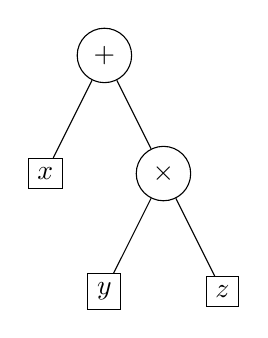
\begin{tikzpicture}
\node [circle,draw] {$+$}
  child {node [draw] {$x$}}
  child {
    node [circle,draw] (M) {$\times$}
    child {node [draw]{$y$}}
    child {node [draw]{$z$}}
  };
\end{tikzpicture}
\qquad\qquad
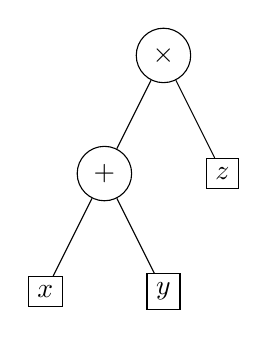
\begin{tikzpicture}
\node [circle,draw] {$\times$}
  child {
    node [circle,draw] (M) {$+$}
    child {node [draw]{$x$}}
    child {node [draw]{$y$}}
  }
  child {node [draw] {$z$}}
;
\end{tikzpicture}
\end{center}

Le regole di interpretazione della precedenza sono convenzionali
e possono esserci situazioni in cui non c'è una completa concordanza su come
una formula vada interpretata.
Quando le formule vengono rappresentate graficamente, inoltre,
anche la presentazione tipografica concorre nell'interpretazione
dell'ordine delle operazioni.
L'uso di spaziature, dimensioni e stili diversi oltre alla
posizione spaziale bidimensionale (linee di frazione, incolonnamenti)
intendono facilitare
l'interpretazione corretta dell'albero di valutazione riducendo
la necessità di utilizzare le parentesi.
\begin{comment}
Esempi di formule di dubbia interpretazione in
cui l'uso delle parentesi sarebbe invece auspicabile:
\[
  x/2\,y,\qquad
  \sin x \cdot 2, \qquad
  {e^x}^2, \qquad
  \frac{\displaystyle\frac{x}{y}}{z}.
\]
\end{comment}

\section{calcolo dei predicati, quantificatori}

Possiamo pensare ai \myemph{predicati} come a proposizioni in cui
compaiono delle variabili.
Se una proposizione ha un valore di verità ben definito, il predicato
ha invece un valore di verità che dipende dal valore assegnato alle sue
variabili. Le variabili da cui dipende un predicato vengono chiamate
\myemph{variabili libere}. Le variabili libere possono venire \emph{chiuse}
(rese \emph{mute}) mediante operatori che agiscono
(estraendo un dato di sintesi) al variare della variabile su tutti i
suoi possibili valori.
Per quanto riguarda il calcolo proposizionale la chiusura delle variabili
di un predicato può essere fatta tramite i \myemph{quantificatori}
\emph{universale} $\forall$ (leggi: ``per ogni'') ed
\emph{esistenziale} $\exists$ (leggi: ``esiste'').
Ad esempio il predicato
$n>5 \Rightarrow n>m$ ha due variabili libere: $n$ ed $m$.
Possiamo chiudere la variabile $n$ con il quantificatore universale ottenendo:
\[
  \forall n \colon n>5 \Rightarrow n>m
\]
che è un predicato con una unica variabile libera $m$.
Il predicato può essere letto così: "per ogni $n$ se $n$ è maggiore di $5$ allora $n$ è anche maggiore di $m$."
Il valore di verità di questo
predicato dipende dal valore assegnato ad $m$.
Più precisamente il predicato è vero se $m\le 5$ ed è falso altrimenti.
La variabile $n$ è invece diventata muta, che significa che non ha più senso
assegnare dei valori alla variabile $n$ in quanto la verità di tale predicato non dipende più da $n$.

Per quanto riguarda l'intepretazione,
la proposizione ottenuta mediante un quantificatore universale
$\forall x\colon P(x)$ è vera se $P(x)$ è vera per ogni possibile valore
assegnato alla variabile $x$ ed è invece falsa se c'è anche un solo valore che
assegnato a $x$ rende falsa $P(x)$. Viceversa nella quantificazione
esistenziale $\exists x\colon P(x)$ si ottiene il vero nel caso ci sia almeno
un valore di $x$ che renda vera $P(x)$ e si ottiene il falso nel caso non ci sia
invece nessun valore di $x$ che renda vera $P(x)$.

Valgono in effetti le seguenti regole formali di scambio dei quantificatori con
la negazione logica:
\begin{align*}
  \neg \forall x \colon P(x) &\iff \exists x \colon \neg P(x)\\
  \neg \exists x \colon P(x) &\iff \forall x \colon \neg P(x).
\end{align*}
Osserviamo che queste relazioni corrispondono alle leggi di De Morgan per lo
scambio della negazione con gli operatori logici di congiunzione e disgiunzione.
Infatti l'operatore universale $\forall$ corrisponde ad una congiunzione logica
$\wedge$ su tutti i possibili valori del predicato,
così come l'operatore esistenziale
$\exists$ corrisponde ad una disgiunzione logica $\vee$.
Dal punto di vista mnemonico osserviamo che i simboli $\exists$ e $\forall$
si ottengono ruotando di 180 gradi le iniziali delle parole
\emph{Esiste} e \emph{Alle} essendo stati introdotti dai matematici Peano e Gentzen.

Una variante dell'operatore esistenziale è l'operatore di unicità:
la proposizione $\exists! x\colon P(x)$ significa che esiste un \emph{unico} valore di $x$
che rende vero il predicato $P(x)$. Formalmente:
\[
  \exists!x\colon P(x) \iff \exists x\colon P(x)
  \wedge \neg \exists y\colon (y \neq x) \wedge P(y).
\]
Osserviamo che la precedente definizione utilizza il simbolo $\neq$ che è la
negazione dell'operatore di uguaglianza $=$ che verrà introdotto nella sezione
seguente.

\section{teoria degli insiemi}

Fin'ora abbiamo presentato le regole logiche per la manipolazione dei valori di
verità dei predicati. Non abbiamo però ancora costruito nessun predicato né
tantomeno abbiamo introdotto gli oggetti che i predicati dovrebbero descrivere.

La teoria degli insiemi serve ad introdurre un \emph{universo} all'interno del
quale potremo identificare degli oggetti che possano rappresentare gli enti
matematici: numeri, funzioni, relazioni, insiemi.
Vedremo però che tutti questi enti matematici potranno essere ricondotti al
concetto di insieme: sarà dunque questo il concetto fondamentale che vogliamo
descrivere.

Intuitivamente gli \myemph{insiemi} sono collezioni di elementi.
Per costruire un sistema formale che descriva gli insiemi sarà sufficiente
introdurre l'unico predicato che mette in relazione un elemento con l'insieme
che lo contiene:
\[
  x \in A
\]
(leggi: ``$x$ è un elemento di $A$``).
Indicheremo con $\not \in$ la negazione
di questa relazione.
Dovremo indicare quali sono le regole formali che ci permetteranno di manipolare
questo tipo di formule.
Sarà utile poter costruire insiemi di insiemi, quindi in realtà nel predicato precedente
$x$ potrebbe a sua volta essere un insieme. Dunque, per semplicità, supporremo
che tutti gli oggetti siano insiemi.

A partire dalla relazione di \myemph{appartenenza} $\in$ potremo definire le altre
relazioni tra insiemi:
\begin{align*}
  A \subset B &\iff \forall x\colon (x \in A \Rightarrow x \in B)\\
  A \supset B &\iff \forall x\colon (x \in A \Leftarrow x \in B)\\
  A = B & \iff A\subset B \,\wedge\, B\subset A.
\end{align*}

Il simbolo $\subset$ rappresenta l'\myemph{inclusione} tra insiemi.
Osserviamo che in altri testi potrà essere invece utilizzato il simbolo $\subsetstrict$
per rappresentare la stessa relazione.

La terza delle regole precedenti si chiama \emph{assioma di estensionalità}
e definisce il fondamentale concetto di \myemph{uguaglianza}.
Il nostro sistema formale sarà dotato di opportune regole di inferenza che
garantiscano che se due oggetti sono uguali
potranno essere liberamente sostituiti uno con l'altro in qualunque
altra formula. Questo garantisce la proprietà transitiva dell'uguaglianza.
Si definirà la \myemph{disuguaglianza} $\not =$ come negazione dell'uguaglianza.

Se $A\subset B$ diremo che $A$ è un \myemph{sottoinsieme} di $B$. Se $A\subset B$ e $A\neq B$ diremo che $A$ è un \emph{sottoinsieme proprio}.

Vogliamo anche introdurre le usuali operazioni di \index{intersezione}\mymargin{intersezione}%
\emph{intersezione} $A\cap B$,
\emph{unione}  $A\cup B$
\index{unione}\mymargin{unione}%
e \emph{differenza} $A \setminus B$
che possono essere codificate dai seguenti assiomi:
\index{differenza tra insiemi}\mymargin{differenza}%
\begin{align*}
  x \in A \cap B &\iff (x \in A \wedge x \in B)\\
  x \in A \cup B &\iff (x \in A \vee x \in B)\\
  x \in A \setminus B &\iff x \in A \wedge x \not \in B.
\end{align*}

Più in generale possiamo richiedere di poter fare l'unione o l'intersezione
di una famiglia $\F$ non vuota di insiemi (una \emph{famiglia} di insiemi non è altro che un insieme di insiemi):
\begin{align*}
  x \in \bigcap \F &\iff \forall A \in \F\colon x \in A \\
  x \in \bigcup \F &\iff \exists A \in \F\colon x \in A.
\end{align*}
Spesso si usano le seguenti notazioni più espressive:
\[
 \bigcap \F = \bigcap_{A \in \F} A,\qquad
 \bigcup \F = \bigcup_{A \in \F} A.
\]

Per avere un primo oggetto su cui agire definiamo l'\myemph{insieme vuoto},
denotato
dal simbolo $\emptyset$, mediante il seguente assioma
\[
\neg \exists x \colon x \in \emptyset.
\]
Osserviamo che le operazioni definite in precedenza, se applicate all'insieme vuoto,
non ci permettono di ottenere nuovi insiemi.
Per avere insiemi con un solo elemento introduciamo l'insieme \myemph{singoletto}
$\{ y \}$ cioè un insieme contenente un unico oggetto $y$:
\[
  x \in \{ y \} \iff x = y.
\]
A questo punto utilizzando l'unione possiamo già ottenere,
per elencazione,
insiemi con un numero
arbitrario (ma finito) di elementi, ad esempio:
\[
  \{a, b, c\} = \{ a \} \cup \{ b\} \cup \{c\}.
\]

Con le operazioni che abbiamo introdotto è già possibile descrivere infiniti insiemi
tra loro diversi. Ad esempio questi sono quattro insiemi diversi:
\[
 \emptyset,\quad
 \{ \emptyset \},\quad
 \{\{\emptyset\}, \emptyset\},\quad
 \{\{\emptyset\}, \{\{\emptyset\}\}\}
\]
mentre ognuno dei seguenti coincide con uno (quale?) dei precedenti:
\[
 \{\emptyset, \emptyset\},\quad
 \{\{\emptyset, \{\emptyset\}\}, \{\{\emptyset\}, \emptyset\}\}.
\]

Possiamo anche definire un insieme mediante una qualunque
proprietà che caratterizzi
i suoi elementi. Se $A$ è un insieme e $P(x)$ un predicato, allora
possiamo definire un insieme $B = \{x\in A\colon P(x)\}$
(si legga: ``$B$ è l'insieme degli $x$ in $A$ tali che vale $P(x)$'')
in modo
che si abbia
(\myemph{assioma di specificazione}):
\[
  b \in \{x\in A \colon P(x)\} \iff (b \in A) \wedge P(b).
\]
Osserviamo che viene richiesto a priori un insieme ambiente $A$ sul quale
viene ristretta la caratterizzazione. Questo significa che questo assioma non
può generare insiemi più grandi di quelli già esistenti.
Questo vincolo si è reso necessario per ovviare al paradosso di Russell.

\begin{paradox}[Russel]
Si consideri l'insieme
\[
  R = \{ x\colon x \not\in x\}.
\]
Allora $R\in R \iff R\not \in R$. Assurdo.
\end{paradox}

Il paradosso di Russel può essere espresso anche nel linguaggio naturale.
Una delle sue accezioni più note si chiama \emph{Paradosso del barbiere}
e si enuncia come segue. Il \emph{barbiere} è quella persona che fa la barba
alle persone che non se la fanno da se. Il barbiere si fa la barba da se?

Con la nostra impostazione l'insieme $R$ di Russel non può essere definito.
Se però fissiamo un insieme \emph{ambiente} $U$, possiamo definire il seguente:
\[
  R = \{ x \in U \colon x \not \in x\}.
\]
In tal caso abbiamo che $R\in R$ se e solo se $(R\in U) \land (R\not \in R)$.
In particolare se fosse $R\in R$ avremmo un assurdo.
%
%
\footnote{%
La relazione $x\in x$ potrebbe di per se sembrare contraddittoria.
Come è possibile che un insieme contenga se stesso come elemento?
Se ad esempio avessimo $x=\{ x\}$ si avrebbe $x=\{\{x\}\} = \{\{\{ x\}\}\} \dots$
e così via in una discesa infinita che non avrebbe mai termine.
La possibilità che esistano insiemi di questo tipo è piuttosto fastidiosa ed è per questo
che si pone l'assioma di \emph{fondazione} (o di \emph{regolarità}) che afferma
in particolare che non esistono insiemi $x$ tali che $x\in x$.
Più in generale l'assioma di fondazione evita che sia possibile
costruire una catena discendente infinita di insiemi che siano
elemento uno dell'altro:
\[
  \dots \in x_n \in \dots \in x_2 \in x_1.
\]
Osserviamo però che anche assumendo che $x\not\in x$ sia sempre vera,
il paradosso di Russel rimane valido, in tal caso infatti
$R=\{x\colon x\not \in x\}$ dovrebbe contenere
tutti gli insiemi e quindi dovrebbe essere $R\in R$... che abbiamo escluso.
}
%
%
Ma non è invece
assurdo che $R\not \in R$, infatti in tal caso potrà essere (anzi, dovrà essere)
$R\not \in U$.
Non abbiamo ottenuto un paradosso, ma abbiamo scoperto che dato
un qualunque insieme $U$ esiste un insieme $R$ che non sta in $U$.
Questo significa che non esiste l'insieme \myemph{universo}, cioè un insieme che
contiene tutti gli insiemi. Osserviamo che l'insieme universo sarebbe il complementare
dell'insieme vuoto, e questo è il motivo per cui non è possibile definire
il complementare di un insieme ma ci si limita a definire la differenza tra insiemi.

Un altro modo per dimostrare che è sempre possibile costruire un
insieme \emph{più grande} di un insieme dato si ottiene dall'insieme potenza
(che vediamo subito) tramite il teorema di Cantor (che vedremo più avanti).

L'assioma dell'insieme potenza, serve
a garantire l'esistenza del\-l'\myemph{insieme delle parti}.
Se $X$ è un qualunque insieme si può considerare $\P(X)$ come l'insieme dei
sottoinsiemi di $X$:
\[
 A \in \P(X) \iff A \subset X.
\]
L'insieme $\P(X)$ si chiama anche \emph{insieme potenza} e viene a volte indicato con $2^X$
in quanto se $X$ ha $n$ elementi allora $\P(X)$ ha $2^n$ elementi.
Ad esempio se $X=\{a, b, c\}$ ha tre elementi, l'insieme delle parti
ha otto elementi:
\[
 \P(X) = \{ \{\}, \{a\}, \{b\}, \{c\}, \{a,b\},
   \{a,c\}, \{b,c\}, \{a,b,c\}\}.
\]
Inteso che $\{\}=\emptyset$ osserviamo che l'insieme vuoto è sottoinsieme di
qualunque altro insieme (verificarlo tramite la definizione),
dunque appartiene sempre all'insieme delle parti.
L'insieme delle parti risulta fondamentale per poter esprimere
la \emph{logica del secondo ordine} ovvero la possibilità di poter
formulare predicati sui sottoinsiemi di un insieme invece che solamente
sui suoi elementi.

\section{relazioni}

Dati $a$ e $b$
definiamo la \myemph{coppia ordinata} $(a,b)$ come un oggetto (un insieme,
visto che abbiamo deciso che tutti gli oggetti matematici sono insiemi) con
la seguente proprietà:
\begin{equation}\label{def:pair}
  (a,b) = (c,d) \iff (a=c) \land (b=d).
\end{equation}
In particolare osserviamo che $(a,b)$ e $(b,a)$ sono diversi tra loro
(a meno che non sia $a = b$) cioè l'ordine in cui vengono elencati i due elementi
è importante.
Formalmente si potrebbe definire $(a,b)=\{\{a\}, \{a,b\}\}$,
si provi per esercizio a dimostrare che con questa definizione vale la
proprietà~\eqref{def:pair}.
Se $A$ e $B$ sono insiemi dati, l'insieme di tutte le coppie di elementi
presi il primo da $A$ e il secondo da $B$ si indica con $A \times B$ e si chiama
\myemph{prodotto cartesiano} di $A$ e $B$:
\[
x \in A \times B \iff \exists a \in A, \exists b \in B\colon x = (a,b).
\]

% Formalmente si potrebbe definire (senza richiedere un nuovo assioma)
% \[
% A \times B = \{X\in \P(\P(A\cup B))\colon \exists a \in A, \exists b \in B \colon X = \{\{a\}, \{a,b\}\}.
% \]

Se $A$ ha $n$ elementi e $B$ ha $m$ elementi, il prodotto $A\times B$ ha $n\cdot m$
elementi. Ad esempio se $A=\{a,b,c\}$ ha tre elementi e $B=\{a,b\}$ ha due elementi,
il prodotto ha sei elementi:
\[
  A \times B = \{(a,a), (a,b), (b,a), (b,b), (c,a), (c,b)\}.
\]

\begin{definition}[relazione]
Una \myemph{relazione} $R$ tra due insiemi $X$ e $Y$ non è altro che un sottoinsieme di $X\times Y$. Più precisamente stiamo quindi parlando di relazioni \emph{binarie}. Per le relazioni binarie il predicato $(x,y)\in R$ viene usualmente scritto con la notazione infissa: $xRy$. La negazione di tale predicato $(x,y)\not \in R$ si scrive usualmente sovrapponendo una barra al simbolo della relazione: $x{\not\! R} y$.

Se $R$ è una relazione tra $X$ e $Y$ si definisce la \myemph{relazione inversa} $R^{-1}$ tra $Y$ e $X$ tramite la seguente definizione:
\[
   x R^{-1} y \iff y R x.
\]
Comunemente si usa anche una riflessione grafica del simbolo, per denotare la relazione inversa: $\reflectbox{$R$} = R^{-1}$.

Se $X=Y$ diremo che $R$ è una relazione su $X$.
Una relazione $R$ su $X$ viene detta
\mymargin{riflessiva\\antiriflessiva\\simmetrica}
\index{relazione!riflessiva}
\index{relazione!antiriflessiva}
\index{relazione!simmetrica}
\emph{riflessiva} se per ogni $x\in X$ si ha $xRx$. Si dice invece \emph{antiriflessiva} se $x\!{\not\!R}x$ per ogni $x\in X$.
La relazione viene detta \emph{simmetrica} se coincide con la sua inversa ovvero se per ogni $x,y\in X$ si ha $xRy \iff yRx$.
Una relazione si dice essere \myemph{antisimmetrica}\index{relazione!antisimmetrica}
 se per
ogni $x,y\in X$ si ha
\[
  x R y \land y R x \implies x=y.
\]
Una relazione si dice essere \myemph{transitiva}
\index{relazione!transitiva}
se
\[
  x R y \land y R z \implies x R z.
\]
\end{definition}

Possiamo pensare ad una coppia $(a,b)$ come ad una freccia che
parte da $a$ e arriva in $b$: $a \mapsto b$.
Potremmo scrivere più espressivamente $(a,b)\in R$ come
$a \stackrel{R}\mapsto b$.
In questo modo una relazione su $A\times B$
risulta essere un insieme di frecce che partono da elementi di $A$
ed arrivano su elementi di $B$. La rappresentazione che si ottiene prende
anche il nome di \emph{grafo orientato}.
Si provi ad interpretare \emph{graficamente} le proprietà
transitiva, simmetrica e riflessiva di un grafo.

Ogni relazione può essere \emph{invertita}\marginpar{relazione inversa}
semplicemente scambiando il ruolo
dei due insiemi $A$ e $B$. Se $R$ è una relazione e vale $x R y$
per la relazione inversa, indicata con $R^{-1}$, si avrà
$y R^{-1} x$.
Pensando ad una relazione $R$ come un insieme di frecce
$x\stackrel R \mapsto y$,
la relazione inversa $R^{-1}$ risulta essere lo stesso insieme di frecce ma
con la direzione opposta $y\stackrel{R^{-1}} \mapsto x$.

\begin{exercise}
Si provi a pensare alla relazione tra persone $xAy$
definita dalla frase "$x$ ama $y$".
Si consideri il significato delle proprietà transitiva, simmetrica
e riflessiva di tale relazione.
\end{exercise}

\section{funzioni}

Le relazioni che più ci interesseranno in questo corso sono le \myemph{funzioni}.
Le funzioni sono le relazioni \emph{univoche} cioè quelle relazioni $f$ in
$A\times B$ che
mandando (nel senso delle frecce) ogni elemento $a\in A$ in uno
ed un solo elemento
$b\in B$:
\[
\forall a\in A\colon \exists ! b\in B\colon a\stackrel{f}\mapsto b.
\]
Tale unico elemento $b\in B$ associato all'elemento $a\in A$ viene chiamato
\emph{immagine} di $a$ tramite $f$ o \emph{valore} di $f$ nel punto $a$ e viene indicato con $b=f(a)$.
Una funzione definita da $A$ in $B$ si indica con $f\colon A \to B$. L'insieme
$A$ viene chiamato \emph{dominio} e l'insieme $B$ \emph{codominio}. \index{dominio}\index{codominio}\mymargin{dominio/codominio}
L'insieme di tutte le funzioni $f\colon A \to B$ viene denotato con $B^A$:
\index{$B^A$}
\[
  B^A = \{f\in \P(A\times B)\colon \text{$f$ è una funzione}\}.
\]
La notazione è giustificata dal fatto che se $A$ ha $n$ elementi e $B$ ha $m$ elementi allora $B^A$ ha $m^n$ elementi.

\begin{exercise}
Si provi a definire le funzioni $\pi_1\colon A \times B \to A$ e $\pi_2\colon A \times B \to B$ che abbiano la proprietà:
\[
   \pi_1(a,b) = a, \qquad \pi_2(a,b) = b.
\]
Le funzioni $\pi_1$ e $\pi_2$ si chiamano proiezioni sul primo e secondo fattore di un prodotto cartesiano e ci permettono di estrarre le componenti di una coppia. Suggerimento: si ricordi che a questo livello una funzione non è altro che un sottoinsieme del prodotto cartesiano: $\pi_1 \subset (A\times B) \times A$, $\pi_2 \subset (A\times B)\times B$.
\end{exercise}


Le funzioni vengono spesso utilizzate per rappresentare delle trasformazioni.
Possiamo pensare ad una funzione come ad una scatola nera (un macinino)
a cui possiamo dare in pasto elementi dell'insieme $A$ (\emph{input})
e otteniamo come risposta elementi dell'insieme $B$ (\emph{output}).

Se l'output (codominio) di una funzione $f$
coincide con l'input (dominio) di una funzione $g$,
cioè se $f\colon A \to B$ e $g\colon B \to C$
possiamo comporre\marginpar{funzione composta}
le due funzioni per ottenere una funzione
$g\circ f \colon A \to C$:
\[
(g\circ f)(x) = g(f(x))\qquad
x \stackrel f \mapsto f(x) \stackrel g \mapsto g(f(x)).
\]

Vedremo come la composizione ci permette di costruire innumerevoli funzioni
componendo tra loro poche funzioni elementari, così come si può costruire un edificio
utilizzando semplici mattoni.
Ovviamente sarà importante conoscere a fondo
tutte le caratteristiche dei mattoni (proprietà delle funzioni elementari)
e sarà pure importante capire come tali proprietà si combinano quando mettiamo
insieme i diversi blocchi.

Uno dei problemi più importanti a
cui si può probabilmente ricondurre qualunque problema
matematico è quello dell'invertibilità di una funzione: data $f\colon A\to B$
trovare una funzione $g\colon B\to A$ tale che
se $x\stackrel f \mapsto y$ allora
$y \stackrel g\mapsto x$. Se ad esempio io so qual è la traiettoria di
un proiettile in funzione dell'angolo di tiro, mi chiedo quale angolo devo
scegliere per centrare un determinato bersaglio.
Oppure (altro esempio) data la funzione $f(x) = x^2$ (definita su un qualche insieme
numerico) dire se è possibile trovare $x$ tale che $f(x) = 2$
(definizione della radice quadrata).
Oppure ancora: se $x A y$ è la relazione ``$x$ ama $y$''
e se io sono $y$ sarei interessato a trovare gli $x$ tali che $x A y$.

Per poter invertire una funzione $f\colon A \to B$ abbiamo la necessità di verificare due
differenti proprietà: che per ogni $b\in B$ esista un elemento $a\in A$ tale che $f(a)=b$
(surgettività)
e che tale elemento $a$ sia unico (iniettività).
Più precisamente diremo che $f\colon A\to B$ è \myemph{surgettiva} se
\[
  \forall b\in B\colon \exists a \in A \colon f(a) = b
\]
ed è \myemph{iniettiva} se
\[
 \forall a\in A, \forall a'\in A\colon (f(a) = f(a') \implies a=a').
\]
Se una funzione $f\colon A \to B$ è iniettiva e surgettiva allora
si dice che $f$ è \myemph{bigettiva} o \emph{invertibile}.
La funzione $g\colon B \to A$ che ad ogni
$b\in B$ associa l'unico $a\in A$ tale che $f(a)=b$ si chiama
\emph{funzione inversa} di $f$.
Tale funzione $g$ si indica anche con il simbolo $f^{-1}$ ed ha le proprietà
\[
  \forall x \in A\colon g(f(x)) = x, \qquad
  \forall y\in B\colon f(g(y)).
\]
In effetti è facile osservare che la funzione inversa $f^{-1}$, vista come relazione, è la relazione inversa di $f$. In generale ogni funzione ha una relazione inversa, ma solo per le funzioni invertibili la relazione inversa è anch'essa una funzione.
La funzione inversa di $f$ è quindi anch'essa invertibile e l'inversa dell'inversa
è $f$ stessa: $(f^{-1})^{-1} = g^{-1} = f$.

Se $f\colon X\to Y$ è una funzione e se $A\subset X$ si definisce
l'insieme $f(A)$, chiamato \myemph{immagine} di $A$ tramite $f$ come:
\[
  f(A) = \{f(x)\colon x \in A\}
\]
se invece $B\subset Y$ si definisce l'insieme $f^{-1}(B)$, chiamato
\myemph{controimmagine} di $B$ tramite $f$ come:
\[
  f(B) = \{x\in A \colon f(x) \in B\}.
\]
Notiamo innanzitutto che la prima definizione non rientra esattamente
nell'assioma di specificazione ma è un modo più immediato per intendere
la seguente definizione che è invece perfettamente valida:
\[
  f(A) = \{y\in B \colon \exists x\in A \colon f(x) = y\}.
\]
Notiamo inoltre che questa definizione rappresenta un \emph{abuso di notazione}.
Infatti avevamo già dato una definizione per il simbolo $f(x)$.
Questa notazione va quindi utilizzata solo se il contesto rende chiaro il fatto
che $A$ va inteso come un sottoinsieme del dominio di $f$ e non come un elemento
di tale dominio.

Se $A=X$ è l'intero dominio della funzione
l'insieme $f(X)$ si chiama \emph{immagine di $f$}.
Possiamo allora osservare che una funzione $f\colon X \to Y$ risulta essere
surgettiva se e solo se $f(X) = Y$.
Se prendiamo un qualunque $y\in Y$ possiamo considerare l'insieme $f^{-1}(\{y\})$
che è sempre definito, anche se $f$ non fosse invertibile. Se tale insieme ha sempre
almeno un elemento significa che la funzione è surgettiva. Se tale insieme ha
sempre non più di un elemento significa che la funzione è iniettiva.
Se tale insieme ha sempre esattamente un elemento allora la funzione è invertibile
e si ha $f^{-1}(\{y\}) = \{f^{-1}(y)\}$.

Questo abuso di notazione
(inserire un insieme dove dovrebbe starci un singolo elemento)
potrà essere utilizzato anche con gli operatori infissi.
Una operazione, rappresentata ad esempio dal simbolo $+$, può essere pensata
come ad una funzione che agisce su una coppia di valori: $+\colon X\times Y \to Z$.
La notazione $x+y$ serve quindi ad abbreviare la notazione $+(x,y)$.
Anche in questo caso potrà capitare che al posto di $x$ o di $y$ o di entrambi,
si inserisca un insieme di valori:
\begin{align*}
   A + y &= \{x+y\colon x \in A\}, \\
   x + B &= \{x+y\colon y \in B\}, \\
   A + B &= \{x+y\colon x\in A, y \in B\}.
\end{align*}
In tutti questi casi il risultato è un insieme di valori, invece che un singolo
valore.

In maniera simile, questo abuso viene attuato anche con le relazioni.
Se ad esempio abbiamo
una relazione $\le$, e $A, B$ sono insiemi, si potrà intendere
che valgano le seguenti notazioni:
\begin{align*}
  x \le B &\iff (\forall y\in B\colon x\le y), \\
  A \le y &\iff (\forall x\in A\colon x \le y), \\
  A \le B &\iff (\forall x\in A, \forall y\in B\colon x\le y).
\end{align*}

\section{numeri naturali}

I numeri naturali rappresentano la prima astrazione matematica che ci viene insegnata fin dalla scuola elementare. L'operazione fondamentale che caratterizza i numeri naturali è il "contare". C'è un primo numero, che per noi sarà lo $0$ (altri testi scelgono $1$ come primo numero naturale) e dato un numero naturale $n$ sarà definito un numero successivo che è quello che usualmente chiamiamo $n+1$. I numeri naturali sono, informalmente, tutti i numeri che si possono ottenere con l'operazione del contare, ovvero partendo da $0$ e passando da ogni numero al successivo.

Nella seguente definizione la funzione $\sigma$ rappresenta il "contare": $\sigma(n)$ è il numero successivo ad $n$. Quando avremo definito l'addizione e il numero $1$, si avrà $\sigma(n) = n+1$.

\begin{definition}[assiomi di Peano]\label{def:naturali}
Sia $\NN$ un insieme e $\sigma\colon \NN\to\NN$ una funzione.
Diremo che $\NN$ soddisfa gli assiomi di Peano con $\sigma$ come funzione \emph{successore} se valgono le seguenti proprietà:
\begin{enumerate}
\item $\sigma$ è iniettiva;
\item esiste un unico elemento $0\in \NN$ (chiamato \emph{zero}) tale che $0\not \in\sigma(\NN)$;
\item (induzione) se $A\subset \NN$, $0\in A$ e $\sigma(A)\subset A$, allora $A=\NN$.
\end{enumerate}
\end{definition}

Se $\NN$ soddisfa gli assiomi di Peano con $\sigma$ come funzione \emph{successore} e $0\not\in\sigma(\NN)$ si potranno definire:
\begin{gather*}
   1 = \sigma(0), \qquad
   2 = \sigma(1), \qquad
   3 = \sigma(2), \qquad
   4 = \sigma(3), \qquad
   5 = \sigma(4), \\
   6 = \sigma(5), \qquad
   7 = \sigma(6), \qquad
   8 = \sigma(7), \qquad
   9 = \sigma(8).
\end{gather*}
Per dare un nome ai naturali ancora successivi si utilizzerà la rappresentazione decimale, certamente nota al lettore, ma che potrà essere formalizzata solo più avanti quando avremo definito le operazioni di addizione, moltiplicazione ed elevamento a potenza.

Gli elementi di $\NN$ saranno chiamati \emph{numeri naturali} (o più semplicemente: naturali).
La funzione $\sigma$ manda quindi un numero naturale nel suo \emph{successore}. Il primo assioma di Peano ci garantisce che naturali diversi hanno successori diversi. Il secondo assioma ci garantisce che ogni naturale tranne $0$ è successore di un altro naturale. Il terzo assioma ci garantisce che partendo da $0$ e iterando la funzione successore si ottengono tutti i numeri naturali.

Il \myhref{https://it.wikipedia.org/wiki/Paradosso_del_Grand_Hotel_di_Hilbert}{paradosso dell'Hotel Hilbert}
mette in evidenza una proprietà apparentemente paradossale dei numeri naturali. A ben guardare questa proprietà paradossale è
dovuta al fatto che la funzione $\sigma \colon \NN \to \NN$ è una funzione iniettiva ma non suriettiva. Quindi $\NN$ può essere messo in corrispondenza biunivoca con un suo sottoinsieme proprio, in quanto $\sigma \colon \NN \to \NN\setminus\{0\}$ è una biezione.

Questa caratteristica viene assunta nella seguente definizione.

\begin{definition}
Diremo che un insieme $A$ è \emph{infinito} se esiste una funzione $f\colon A \to A$ iniettiva ma non suriettiva. Diremo che un insieme è \emph{finito} se non è infinito ovvero se ogni funzione iniettiva $f\colon A \to A$ è anche suriettiva.
\end{definition}

L'insieme dei numeri naturali è dunque un insieme infinito. Ma nessuno degli assiomi cha abbiamo finora preso in considerazione garantisce l'esistenza di un qualche insieme infinito. Anzi, si potrebbe osservare che un eventuale universo formato solamente da insiemi finiti soddisfa tutti gli assiomi della teoria degli insiemi che abbiamo finora considerato. E' quindi necessario stipulare l'esistenza dei numeri naturali (o almeno di un qualunque insieme infinito) per assioma.

\begin{axiom}[assioma di infinito]
Esiste un insieme infinito.
\end{axiom}

\begin{theorem}[$\NN$ è il più piccolo insieme infinito]
\label{th:minimo_infinito}
Se $A$ è un insieme infinito esiste $N\subset A$ e $\sigma\colon N\to N$ tale che $N$ soddisfa gli assiomi di peano rispetto alla funzione $\sigma$.
\end{theorem}
%
\begin{proof}
Per definizione se $X$ è un insieme infinito significa che esiste $f\colon X \to X$ iniettiva ma non suriettiva. Fissiamo $0\in X\setminus \sigma(X)$ e diciamo che un sottoinsieme $A\subset X$ è \emph{induttivo} se $0\in A$ e $f(A)\subset A$.
Definiamo quindi
\begin{align*}
  \mathcal F &= \{A\in \mathcal P(X)\colon \text{$A$ induttivo}\}\\
  N &= \bigcap \mathcal F.
\end{align*}
Ovviamente $X\in \mathcal F$, dunque $\mathcal F$ non è vuoto. Visto che per definizione di insieme induttivo $0$ è elemento di ogni insieme induttivo deduciamo che $0\in N$.
Vogliamo mostrare anche che $f(N)\subset N$: preso $n\in N$ sappiamo che, per definizione, $n$ è elemento di tutti i sottoinsiemi induttivi di $X$. Ma allora anche $f(n)$ è elemento di ogni insieme induttivo e dunque $f(n)\in N$. Posto $\sigma = f_{|N}$ ($\sigma$ è la restrizione di $f$ ad $N$) otteniamo che $\sigma\colon N\to N$ è iniettiva (il primo assioma di Peano) e $0\not \in \sigma(N)$. Per avere il secondo assioma di Peano dobbiamo dimostrare che $0$ è l'unico elemento di $N\setminus \sigma(N)$. Supponiamo per assurdo che esista $n\in N\setminus \sigma(N)$, $n\neq 0$. Allora l'insieme $A=N\setminus\{n\}$ è un insieme induttivo di $X$ in quanto $0\in A$ e $s(A) = \sigma(A) \subset N\setminus\{n\} = A$. Dunque $A\in \mathcal F$ e, per come abbiamo definito $N$, dovrà essere $N \subset A$. Ma questo è assurdo perché $n\in N$ ma $n\not \in A$. Per concludere la dimostrazione dobbiamo dimostrare che vale anche il terzo assioma di Peano. Sia dunque $A\subset N$ tale che $0\in A$ e $\sigma(A)\subset A$: significa che $A\in \mathcal F$ e quindi $N\subset A$, come richiesto.
\end{proof}

D'ora in poi denoteremo con $\NN$ un insieme che soddisfa gli assiomi di Peano. Per l'assioma di infinito e grazie al Teorema~\ref{th:minimo_infinito} è garantita l'esistenza di tale insieme.

La proprietà induttiva dei numeri naturali permette di definire
una funzione su $\NN$ utilizzando la cosiddetta
\myemph{definizione per induzione} (o \emph{definizione ricorsiva}).

\begin{theorem}[definizione per induzione]%
\label{th:def_induction}
Sia $X$ un insieme, $x_0 \in X$, $g\colon X \to X$. Allora esiste una unica funzione $f\colon \NN \to X$ tale che
\[
  \begin{cases}
    f(0) = x_0 \\
    f(\sigma(n)) = g(f(n)).
  \end{cases}
\]

Più in generale se $g\colon \NN \times X \to X$
esisterà una unica $f\colon \NN \to X$ tale che
\begin{equation}\label{eq:def_induction_non_auto}
\begin{cases}
  f(0) = x_0 \\
  f(\sigma(n)) = g(n, f(n)) \qquad \forall n\in \NN.
\end{cases}
\end{equation}
\end{theorem}

Intuitivamente dopo aver definito $f(0) = x_0$ si potrà definire
$f(1) = g(0, f(0))$, $f(2) = g(1, f(1))$, $f(3) = g(2, f(2))$ etc.
Per la proprietà induttiva dei numeri naturali la funzione $f$ risulterà
definita univocamente su tutti i numeri naturali.

\begin{proof}[Dimostrazione del Teorema~\ref{th:def_induction}]
Dimostriamo direttamente il caso più generale. Consideriamo
l'insieme
\[
  \Gamma = \{ G \subset \NN \times X\colon (0,x_0)\in G,
  (n,x)\in G \implies (\sigma(n), g(n, x)\in G\}.
\]
L'insieme $\Gamma$ contiene tutte le relazioni che soddisfano  \eqref{eq:def_induction_non_auto}. Possiamo sperare di ottenere una funzione
prendendo la più piccola relazione:
\[
   f = \bigcap \Gamma = \bigcap_{G\in \Gamma} G.
\]
E' chiaro che $f\in \Gamma$.
Dimostriamo che $f$ è una funzione. Innanzitutto mostriamo che $f$ è definita su tutto $\NN$: sia $D=\{n\in \NN \colon \exists x\in X \colon (n,x)\in f\}$ il dominio della relazione $f$. Certamente $0\in D$ in quanto $(0,x_0)\in G$ per ogni $G\in \Gamma$ e quindi $(0,x_0)\in f$. Inoltre se $n\in D$ allora esiste $x\in X$ tale che $(n,x)\in f$. Significa che $(n,x)\in G$ per ogni $G\in \Gamma$. Ma per come è definito $\Gamma$ significa che anche $(\sigma(n),g(n,x))\in G$ per ogni $G\in \Gamma$. Dunque $(\sigma(n),g(n,x))\in f$ e $\sigma(n)\in D$. Ma allora per il principio di induzione possiamo dedurre che $D=\NN$. Vogliamo ora mostrare che $f$ è univoca: consideriamo l'insieme
\[
  A = \{n\in \NN \colon \exists x,y\in X \colon x \neq y \land (n,x)\in f \land (n,y) \in f\}.
\]
L'insieme $A$ rappresenta i numeri naturali sui quali $f$ non è univoca.
Se $A$ non è vuoto allora $A$ ammette minimo: sia $m$ il minimo di $A$.
Se $m=0$ scelto $x\in X$ tale che $(0,x)\in f$ possiamo togliere $(0,x)$ da $f$ e ottenere una relazione $G=f\setminus\{(m,x)\}$ che sta ancora in $\Gamma$.
Ma questo è assurdo in quanto dovrebbe essere $f\subset G$. Se invece $m\neq 0$ allora esiste $m'$ tale che $\sigma(m')=m$ (cioè, intuitivamente, $m'=m-1$) e visto che $f$ è definita su $m'$ ed è univoca su $m'$ esiste un unico $x'$ tale che $(m',x')\in f$. Allora posto $x=g(m',x')$ si ha $(m,x)\in f$. Visto che $f$ non è univoca su $m$ esiste $y\neq x$ tale che anche $(m,y)\in f$. E' chiaro allora che possiamo togliere il punto $(m,y)$ da $f$ e ottenere una relazione $G=f \setminus\{(m,y)\}$ che è ancora in $\Gamma$. Ma dovrebbe essere $f\subset G$ che è assurdo.
\end{proof}

Come prima applicazione della definizione per induzione possiamo definire cosa si intende per \emph{iterata} di una funzione. Intuitivamente se $f\colon A \to A$ è una qualunque funzione, vorremmo definire:
\[
  f^n \colon A \to A
\]
come la funzione $x \mapsto \overbrace{f( \dots (f(f(x))))}^{\text{$n$ volte}}$ dove al posto dei puntini $\dots$ si dovranno inserire tante $f$ in modo da averne $n$ in totale.

\begin{definition}
Sia $f\colon A \to A$ una funzione e sia $n\in \NN$ un numero naturale.
Si definisce allora $f^n\colon A \to A$ per induzione su $n$ in modo
che per ogni $a\in A$ si abbia:
\[
\begin{cases}
  f^0(a) = a \\
  f^{\sigma(n)}(a) = f(f^n(a)) \\
\end{cases}
\]
\end{definition}

L'iterata $f^n$ è ben definita in base al Teorema~\ref{th:def_induction}. Infatti si può considerare l'insieme $H=A^A$ delle funzioni $h\colon A\to A$ e la funzione $F\colon H\to H$ definita da $F(h) = f\circ h$. Partendo dal punto $h_0\colon A\to A$, $h_0(a)=a$ (la funzione identità) si definirà quindi $f^0 = h_0$, $f^{\sigma(n)} = G(f^n)$.

Tramite le iterate vorremmo ora definire le operazioni di somma, prodotto e potenza. Innanzitutto definiamo cosa si intende per \emph{operazione}.

\begin{definition}[operazione]\label{def:operazione}
Una funzione $*\colon X \times Y \to Z$ si dice essere una
\myemph{operazione} (o più precisamente: una operazione binaria, visto che opera su una coppia). Per le operazioni binarie si utilizzerà abitualmente la notazione infissa:
\[
  x * y = *(x,y).
\]

Nel caso $X=Y=Z$ diremo che $*$ è una operazione su $X$.
In tal caso diremo che l'operazione è \myemph{associativa} se per ogni $x,y,z\in X$ vale la seguente proprietà:
\[
   (x*y)*z = x*(y*z).
\]
Diremo che l'operazione è \myemph{commutativa} se per ogni $x,y\in X$ vale la seguente proprietà:
\[
  x*y = y*x.
\]
Diremo che $e\in X$ è un \myemph{elemento neutro} per l'operazione $*$ se per ogni $x\in X$ valgono le seguenti proprietà:
\[
  x * e = e * x = x.
\]
Se esiste un unico elemento neutro, $e$, diremo che $x$ è l'\myemph{inverso} di $y$ per l'operazione $*$ se vale:
\[
  x*y = y*x = e.
\]
E' facile\footnote{%
Infatti se $y$ e $z$ fossero due inversi di $x$ si avrebbe da un lato: $y*x*z = e*z = z$ dall'altro $y*x*z = y*e = y$ e dunque $y=z$.
} verificare che se l'inverso esiste è unico.
Se $+$ e $\cdot$ sono due operazioni definite sullo stesso insieme $X$ diremo che vale la proprietà \myemph{distributiva} di $+$ rispetto a $\cdot$ se per ogni $x,y,z\in X$  valgono le seguenti proprietà:
\[
  (x + y)\cdot z = (x\cdot z) + (y\cdot z), \qquad
  x\cdot (y + z) = (x\cdot y) + (x\cdot z).
\]
\end{definition}

Possiamo ora definire l'operazione addizione $+$ su $\NN$ in modo che valgano le seguenti proprietà:
\[
   \begin{cases}
     n + 0 = n \\
     n + \sigma(m) = \sigma(n+m)
   \end{cases}
\]
Intuitivamente è chiaro che questa definizione è ben posta per induzione.
Formalmente si tratta di ricondursi al
Teorema~\ref{th:def_induction}. Per fare ciò possiamo definire una funzione
$f\colon \NN \to (\NN\to \NN)$ in modo che sia $f(m)(n) = n+m$
(si noti che i valori della funzione $f$ sono a loro volta funzioni).
La funzione $f$ può essere definita
per induzione come segue:
\[
 \begin{cases}
 f(0) = (n\mapsto n)\\
 f(\sigma(m)) = (n\mapsto \sigma(n+m)).
 \end{cases}
\]

Possiamo finalmente affermare che per ogni $m\in \NN$ si ha $\sigma(m)=m+1$ (basterà porre $n=0$ nell'identità $n+\sigma(m)=\sigma(n+m)$ e usare $n+0=0$).
Dunque d'ora in avanti abbandoneremo il simbolo $\sigma$ per indicare il successore e utilizzeremo solamente l'addizione appena definita.

In particolare ora possiamo dare un enunciato del principio di induzione come usualmente viene utilizzato.

\begin{theorem}[Principio di induzione]
Se $P(n)$ è una proposizione che dipende da una variabile $n\in \NN$ e se valgono le seguenti proprietà:
\begin{enumerate}
\item $P(0)$;
\item $\forall n\in \NN\colon P(n) \implies P(n+1)$
\end{enumerate}
allora vale
\[
  \forall n\in \NN \colon P(n).
\]
\end{theorem}
\begin{proof}
Se facciamo corrispondere alla proposizione $P$ l'insieme dei numeri su
cui $P$ è valida: $A=\{n\in \NN\colon P(n)\}$ il teorema
si riconduce all'assioma di induzione dei numeri naturali.
\end{proof}

Le operazioni di moltiplicazione $\cdot$ ed elevamento a potenza su $\NN$
si definiscono per induzione in maniera analoga a come abbiamo fatto per l'addizione.
Si richiederà che valgano le seguenti proprietà:
\begin{gather*}
   \begin{cases}
     n + 0 = n \\
     n + \sigma(m) = \sigma(n+m)\\
   \end{cases}
   \qquad
   \begin{cases}
     n \cdot 0 = 0\\
     n \cdot \sigma(m) = (n\cdot m) + m\\
   \end{cases}
   \\
   \begin{cases}
     n ^ 0 = 1\\
     n ^ \sigma(m) = n^m \cdot n.
   \end{cases}
\end{gather*}

Si osservi che abbiamo definito $0^0=1$.
Alcuni testi considerano indefinita tale operazione ma
questa è una definizione del tutto naturale che ci sarà molto comoda nel seguito.

Il principio di induzione ci permette di dimostrare le seguenti proprietà delle
operazioni appena definite.

\begin{theorem}[proprietà delle operazioni elementari]
Le operazioni di addizione e moltiplicazione su $\NN$ hanno elemento neutro
(rispettivamente lo $0$ e l'$1$) soddisfano la proprietà associativa, commutativa
e distributiva. In formule, per ogni $n,m,r\in \NN$ si ha
\begin{gather*}
  n+0= n, \qquad n+(m+r) = (n+m)+r, \qquad n+m=m+n\\
  n\cdot 1 = n, \qquad n\cdot(m\cdot r) = (n\cdot m)\cdot r, \qquad n\cdot m=m\cdot n\\
  n\cdot(m+r) = n\cdot m + n \cdot r.
\end{gather*}
Si dirà inoltre che $0$ è elemento assorbente per la moltiplicazione in quanto si ha
\[
   n\cdot 0 = 0
\]
e inoltre vale la proprietà di annullamento del prodotto:
\[
  n\cdot m = 0 \iff (n=0)\lor(m=0).
\]

L'elevamento a potenza soddisfa le seguenti notevoli proprietà:
\begin{gather*}
n^0 = 1, \qquad
n^{m+r} = n^m \cdot n^r, \qquad
(n^m)^r = n^{m\cdot r}.
\end{gather*}
\end{theorem}

Si noti (facendo qualche semplice esempio)
che l'elevamento a potenza non è associativo né commutativo. Per
convenzione se non vengono utilizzate le parentesi si assume che l'elevamento
a potenza associ verso destra:
\[
  n^{m^r} = n^{(m^r)}.
\]

Come ulteriore esempio di applicazione della definizione per induzione definiamo
il \emph{fattoriale} $n! = 1 \cdot 2 \dots n$ (il prodotto dei numeri naturali
da $1$ a $n$).
Per definire tale funzione
$\NN \to \NN$ in maniera rigorosa osserviamo che il prodotto dei numeri da $1$
a $n+1$ può essere definito come il prodotto dei numeri da $1$ a $n$ moltiplicato
per $n+1$.
Imponendo poi che\footnote{%
E' chiaro che deve essere $1!=1$ e di conseguenza se vale $(n+1)! = (n+1)\cdot n!$
dovrà essere $0!=1$.
D'altra parte è naturale che il prodotto di un insieme vuoto di numeri sia
l'elemento neutro del prodotto, così come la somma di zero numeri è l'elemento
neutro della somma.
}
$0!=1$, si ottiene una caratterizzazione univoca:
\[
 \begin{cases}
  0! = 1 \\
  (n+1)! = (n+1) \cdot n!
 \end{cases}
\]
Si tratta di applicare il Teorema~\ref{th:def_induction}
con $X=\NN$, $\alpha = 1$, $g(n, x) = (n+1)\cdot x$ per garantire che esiste
una unica funzione $\NN\to\NN$, $n\mapsto n!$, che soddisfa queste proprietà.

\begin{definition}[relazione d'ordine]
Una relazione $\le$ su un insieme $X$ si dice essere una
relazione d'\myemph{ordine parziale} (o più semplicemente una relazione d'ordine)
se è riflessiva, antisimmetrica e transitiva.
La relazione inversa si denota con $\ge$ ed è anch'essa una relazione d'ordine.

Se $\le$ è una relazione d'ordine parziale, si denota con $<$
(chiamato ordine stretto) la relazione definita da:
\[
  x < y \iff (x\le y) \land (x\neq y).
\]
La relazione $<$ è anch'essa transitiva e antisimmetrica (la condizione $(x<y)
 \land (y<x)$ non è mai verificata) ma ovviamente non è riflessiva, anzi
 è \myemph{antiriflessiva}: $x\not < x$ per ogni $x\in X$. La relazione inversa
 di $<$ si denota con $>$.

Data una relazione d'ordine $\le$ su $X$ diremo che $x,y\in X$ sono
 \myemph{confrontabili} se vale $x\le y$ oppure $y\le x$
 (dicotomia\index{dicotomia}).
Se tutti gli elementi di $X$ sono confrontabili diremo che la relazione
d'ordine è \emph{totale}\mymargin{ordine totale}. In tal caso vale la
tricotomia: se $x,y\in X$ allora una e una sola delle seguenti proprietà è vera:
\[
  x < y, \qquad x > y, \qquad x=y.
\]
\end{definition}

Sui numeri naturali
si potrà a questo punto definire una relazione $\le$ tramite la condizione
\[
  n \le m \iff \exists k \in \NN \colon m = n+k.
\]

\begin{theorem}
Si ha
\[
 \forall n,m,r\in \NN \colon n\le m \implies n+r \le m+r.
\]
Inoltre
la relazione $\le$ su $\NN$ è una relazione d'ordine totale.
\end{theorem}
\begin{proof}
Per la prima affermazione si tratta solamente di applicare la definizione
di $\le$. Se $m\le n$ allora $n+k = m$ dunque $n+r+k = m+r$
e quindi $m+r\le n+r$.

Per dimostrare che l'ordine $\le$ è totale dobbiamo mostrare che se non esiste
$k$ tale che $n = m+k$ allora esiste $j$ tale che $m=n+j$.
Dato $n$ consideriamo l' ********

Osserviamo ora che $m+k = m$ se e solo se $k=0$. Infatti posto
\[
M=\{m\in \NN\colon m+k = m \implies k=0 \}
\]
si ha chiaramente $0\in M$. E se fosse $(m+1)+k=m+1$ si avrebbe $(m+k)+1=m+1$ e,
per l'iniettività della funzione $\sigma(n)=n+1$ si dovrebbe avere $m+k=m$.
Dunque se $m\in M$ allora anche $m+1\in M$. Per l'assioma di induzione otteniamo
$M=\NN$ e dunque la proprietà che volevamo dimostrare.

Dunque se abbiamo $n\ge m$ e $m\ge n$ significa che esistono $k$ e $j$
tali che $n=m+k$ e $m=n+j$ da cui $n=n+(k+j)$. Ma allora $k+j=0$
\end{proof}

\begin{theorem}[buon ordinamento di $\NN$]
\index{buon ordinamento}
Se $A$ è un sottoinsieme non vuoto di $\NN$ allora esiste $a \in A$
tale che per ogni $x\in A$ si ha $a\le x$ (ovvero $a$ è minimo di $A$).
\end{theorem}
%
\begin{proof}
Supponiamo per assurdo che $A$ non abbia minimo e consideriamo l'insieme
$B=\{b\in \NN\colon b \le A\}$.
Chiaramente $0\in B$ in quanto $0\le \NN$. Se poi sapessimo che $n\in B$
allora $n\le A$. Non può essere $n\in A$ altrimenti $n$ sarebbe il minimo di $A$. Dunque $n < A$ e quindi $n+1 \le A$. Abbiamo quindi mostrato che se $n\in B$ anche $n+1\in B$. Per il principio di induzione deduciamo che $B=\NN$ e quindi $A$ sarebbe vuoto, cosa che abbiamo escluso per ipotesi.
\end{proof}



La relazione $\ge$ si definisce come la relazione inversa di $\le$.
E le relazioni $<$ e $>$ saranno le corrispondenti relazioni d'ordine stretto.

Diremo che un numero $n\in \NN$ è divisibile per $m\in \NN$ se esiste $k\in \NN$
tale che $n = k \cdot m$. In tal caso scriveremo $k = n/m$.



In maniera simile si potrà definire per ogni $n,m \in \NN$ l'elevamento a potenza $n^m$
in modo che valga\footnote{%
Si noti che stiamo definendo $0^0=1$.
Alcuni testi lasciano indefinita questa operazione ma in realtà la formula
è giustificata dal fatto che $0^0$ è un prodotto di $0$ fattori e quindi,
come $0!$, deve valere $1$.
Questo viene confermato dal fatto che $n^m$ è il numero di funzioni da un
insieme con $m$ elementi in un insieme con $n$ elementi e
su un dominio vuoto è definita una unica funzione (la funzione vuota), anche
se il codominio è vuoto.
}
\[
\begin{cases}
  n^0 = 1\\
  n^{m+1} = n\cdot n^m.
\end{cases}
\]

La proprietà induttiva dei numeri naturali è equivalente al seguente.
\begin{theorem}[principio di induzione]
\index{principio di induzione}
\mymargin{principio di induzione}
Sia $P(n)$ un predicato sui numeri naturali $n\in \NN$.
Se valgono le seguenti condizioni
\begin{enumerate}
\item $P(0)$ è vera
\item $P(n) \implies P(n+1)$
\end{enumerate}
allora $P(n)$ è vera per ogni $n\in \NN$.
\end{theorem}
%
\begin{proof}
Si consideri l'insieme $A=\{n\in \NN\colon \text{$P(n)$ è vera}\}$ e si
applichi il terzo assioma di Peano per verificare che $A=\NN$.
\end{proof}

\begin{theorem}[unicità dei numeri naturali]
Se $\NN$ e $\NN'$ sono insiemi di numeri naturali rispetto alle
funzioni $\sigma\colon \NN \to \NN$ e $\sigma'\colon \NN'\to \NN'$
con $0\in \NN\setminus\sigma(\NN)$ e $0'\in \NN'\setminus\sigma'(\NN')$
allora $\NN$ e $\NN'$ sono \emph{isomorfi} nel senso che esiste una
corrispondenzia biunivoca $\phi\colon \NN \to \NN'$ tale che:
\[
  \phi(0) = 0', \qquad \sigma'\circ \phi = \phi\circ \sigma.
\]
\end{theorem}


\begin{exercise}
La somma $S(n) = 1 + 2 + \dots +n$
dei naturali da $1$ fino a $n$ può essere definita come quella unica funzione
che soddisfa le proprietà
\[
\begin{cases}
  S(0) = 0 \\
  S(n+1) = S(n) + (n+1).
\end{cases}
\]
Dimostrare che $S(n) = n \cdot (n+1) / 2$.
\end{exercise}

\begin{exercise}
Dimostrare che per la somma
$Q(n) = 1^2 + 2^2 + \dots + n^2$
(somma dei quadrati dei naturali da $1$ a $n$)
vale la formula
$Q(n) = n \cdot (n+1)\cdot (2n + 1) / 6$.
\end{exercise}

Potrà risultare utile utilizzare le seguenti varianti del principio di
induzione la cui dimostrazione si riconduce facilmente al principio di induzione usuale.
\begin{theorem}[principio di induzione (variante)]
\index{principio di induzione}
Sia $P(n)$ un predicato definito sui numeri naturali $n$
non inferiori a $n_0\in \NN$.
Se
\begin{enumerate}
\item $P(n_0)$ è vero
\item $P(n) \implies P(n+1)$ per ogni $n\ge n_0$
\end{enumerate}
allora $P(n)$ è vero per ogni $n\ge n_0$.
\end{theorem}

\begin{theorem}[principio di induzione forte]
\index{principio di induzione forte}
Sia $P(n)$ un predicato definito sui numeri naturali $n\in \NN$.
Se
\begin{enumerate}
\item $P(0)$ è vero
\item $(\forall k\le n\colon P(k))\implies P(n+1)$
\end{enumerate}
Allora $P(n)$ è vero per ogni $n\in \NN$.
\end{theorem}

\begin{theorem}[buon ordinamento di $\NN$]
\index{buon ordinamento}
Se $A$ è un sottoinsieme non vuoto di $\NN$ allora esiste $a \in A$
tale che per ogni $x\in A$ si ha $a\le x$ (ovvero $a$ è minimo di $A$).
\end{theorem}
%
\begin{proof}
Supponiamo per assurdo che $A$ non abbia minimo e consideriamo l'insieme
$B=\{b\in \NN\colon b \le A\}$.
Chiaramente $0\in B$ in quanto $0\le \NN$. Se poi sapessimo che $n\in B$
allora $n\le A$. Non può essere $n\in A$ altrimenti $n$ sarebbe il minimo di $A$. Dunque $n < A$ e quindi $n+1 \le A$. Abbiamo quindi mostrato che se $n\in B$ anche $n+1\in B$. Per il principio di induzione deduciamo che $B=\NN$ e quindi $A$ sarebbe vuoto, cosa che abbiamo escluso per ipotesi.
\end{proof}

\begin{exercise}
Utilizzando il principio di induzione dimostrare che se $\# A = n$ allora:
\begin{enumerate}
    \item $\# \P(A) = 2^n$;
    \item $\# \{f\colon A \to A\colon \text{$f$ biettiva}\} = n!$
      (le funzioni biettive di un insieme in sé si chiamano anche
      \emph{permutazioni}).
\end{enumerate}
\end{exercise}

\begin{definition}[massimo/minimo, sup/inf]
Sia $\le$ una relazione d'ordine totale su un insieme $X$. Dato $x\in X$ e $A\subset X$ diremo che:
\begin{enumerate}
\item $x$ è un \emph{minorante} di $A$ e scriveremo $x\le A$,
se $x\le a$ per ogni $a \in A$;
$x$ è un \emph{maggiorante} di $a$, $A\le x$, se $a \le x$ per ogni $a \in A$;
\item $A$ è \emph{inferiormente limitato} se ammette un minorante ovvero esiste $x\in X$ tale che $x\le A$; $A$ è \emph{superiormente limitato} se ammette un maggiorante ovvero esiste $x\in X$ tale che $A \le x$; $A$ è \emph{limitato} se è sia superiormente che inferiormente limitato;
\item $x$ è \emph{minimo} di $A$ se $x\in A$ e $x\le A$;
$x$ è \emph{massimo} di $A$ se $x\in A$ e $A \le x$;
\item $x$ è \emph{estremo inferiore} di $A$ se $x$ è massimo dei minoranti;
$x$ è \emph{estremo superiore} di $A$, $x=\sup A$ se $x$ è il minimo dei maggioranti.
\end{enumerate}

In base al teorema seguente il massimo, minimo, estremo superiore e inferiore quando esistono sono unici. Potremo quindi denotarli univocamente con i seguenti simboli:
\[
  \max A,\qquad
  \min A,\qquad
  \sup A,\qquad
  \inf A.
\]
\end{definition}

\begin{theorem}[unicità di $\min$, $\max$, $\inf$, $\sup$]
Massimo, minimo, estremo superiore ed estremo inferiore, se esistono, sono unici.
\end{theorem}
\begin{proof}
**** DA FARE ****
\end{proof}

\begin{definition}[quoziente]
Una relazione $\sim$ su un insieme $X$ si dice essere una \myemph{relazione di equivalenza}
se è riflessiva, simmetrica e transitiva.
\end{definition}

\section{cardinalità}

La teoria degli insiemi è nata con l'intento di formalizzare l'utilizzo degli
insiemi con infiniti elementi. Infatti finché gli insiemi hanno un numero finito
di elementi non ci sono dubbi sulle loro proprietà. L'utilizzo di insiemi con
infiniti elementi, invece, ci pone di fronte a questioni che possono sembrare
paradossali.

Per confrontare gli insiemi finiti è sufficiente contare il numero degli elementi.
Diremo che un insieme è \emph{più grande} se ha un numero di elementi maggiore.
Ma se gli insiemi sono infiniti, non siamo in grado di effettuare un conteggio
degli elementi. Possiamo però osservare che non è necessario contare il numero
di elementi per poter dire che due insiemi hanno la stessa numerosità.
Ad esempio in un parcheggio pieno posso dire che il numero di automobili
è uguale al numero di posti, senza dover contare né l'uno né l'altro ma semplicemente
osservando che c'è una corrispondenza biunivoca tra i posti e le auto. Faremo
lo stesso per confrontare insiemi infiniti.

Diciamo che due insiemi $A$ e $B$ sono \emph{equipotenti} e scriveremo $\#A = \#B$
\index{\#}%
se esiste una funzione bigettiva $f\colon A \to B$.
Il simbolo $\#A$ si chiama \myemph{cardinalità} di $A$ e quindi due insiemi
sono equipotenti se hanno la stessa cardinalità.
In tal caso la funzione
$f$ è invertibile e l'inversa è anch'essa bigettiva,
quindi se $\#A = \#B$ risulta anche $\#B = \#A$.
Tramite la composizione è inoltre facile verificare che se $\#A = \#B$ e $\#B = \#C$
allora $\#A = \#C$.
Nel caso degli insiemi finiti vedremo che la cardinalità coincide con il
numero di elementi dell'insieme, ma ci potranno essere anche cardinalità
\emph{infinite}.

La relazione di equipotenza definisce il concetto di cardinalità, specificando
quali sono gli insiemi che hanno la stessa cardinalità. Possiamo anche mettere
un ordinamento tra gli insiemi, specificando che un insieme $A$ ha cardinalità
minore o uguale a quella di $B$, $\#A\le \#B$, se esiste una funzione
iniettiva $f\colon A \to B$. Scriveremo $\#A < \#B$ per indicare che
$\#A \le \#B$ ma non $\#A = \#B$ (dunque esistono funzioni iniettive da $A$ in $B$
ma nessuna di queste risulta essere surgettiva).

Non è difficile verificare che se esiste una funzione iniettiva $f\colon A\to B$
allora esiste anche una funzione surgettiva $g\colon B\to A$
(basta osservare che una funzione iniettiva $f$ è invertibile sulla propria
immagine $f\colon A \to f(A)$ e la funzione inversa può essere estesa a
tutto $B$ in maniera arbitraria).

Sugli insiemi finiti, di nuovo, questo concetto
si traduce con la corrispondente
disuguaglianza tra il numero degli elementi dei due insiemi.
Sugli insiemi infiniti, invece, abbiamo un concetto nuovo e i seguenti teoremi
non sono scontati.

\begin{theorem}[Cantor-Bernstein]
\index{teorema!di Cantor-Bernstein}
Se $\#A \le \#B$ e $\#B \le \#A$ allora $\#A = \#B$.
\end{theorem}
%
\begin{figure}
  \centering
  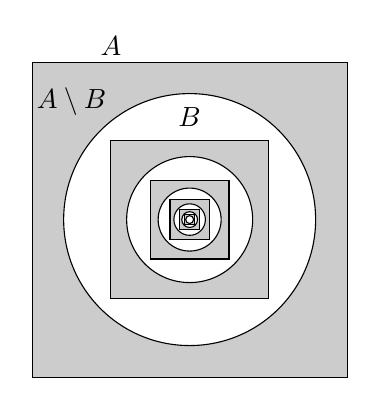
\begin{tikzpicture}
  \foreach \x in {1,0.5,0.25,0.25*0.5,0.25*0.25,0.25*0.25*0.5} {
    \path[draw,fill=black!20] (2*\x,2*\x)--(-2*\x,2*\x)--(-2*\x,-2*\x)--(2*\x,-2*\x)--cycle;
    \draw[fill=white] (0,0) circle (1.6*\x);
  };
  \node at (-1.0,2.2) {$A$};
  \node at (-1.5,1.5) {$A\setminus B$};
  \node at (0,1.3) {$B$};
  \node at (-0.75,0.75) {$$};
\end{tikzpicture}

  \caption{
  Nella dimostrazione del teorema di Cantor-Bernstein
  $A$ è rappresentato da un quadrato e $B$ da un cerchio contenuto
  in $A$. L'immagine di $A$ in $B$ è rappresentata da un quadrato contenuto
  in $B$ e così via. La parte ombreggiata è l'insieme $D$.
  }
  \label{fig:omotetia}
\end{figure}
%
\begin{proof}
Per prima cosa al posto dell'ipotesi $\# B \le \#A$ prendiamo
l'ipotesi apparentemente più forte $B\subset A$.
Vedremo alla fine che questa ipotesi non ci fa perdere di generalità.

Essendo per ipotesi $\#A \le \#B$ esiste $f\colon A \to B$ iniettiva.
Intuitivamente l'idea è quella di definire l'insieme
\[
 D = (A\setminus B)  \cup f(A\setminus B) \cup f^2(A\setminus B) \cup \dots
\]
(si intende $f^2=f\circ f$, $f^3=f\circ f\circ f$ etc...)
e di definire la biezione $\phi \colon A \to B$ mandando ogni "buccia"
$f^n(A\setminus B)$ in $f^{n+1}(A\setminus B)$ e lasciando fisso
il resto di $B$.

Per farlo in maniera rigorosa
consideriamo allora la famiglia di insiemi $\F = \{X \subset A \colon X \supset A \setminus B, f(X) \subset X\}$ e definiamo $D = \bigcap \F$.
Osserviamo che $A \in \F$ quindi $\F\neq \emptyset$.

E' facile verificare che $f(D) \subset D$ infatti dato $x\in D$ per ogni $X\in \F$ deve essere $x\in X$ ma allora $f(x) \in X$ (per come è definito $\F$), dunque $f(x) \in D$. In modo analogo si dimostra che $D\supset A\setminus B$ e dunque concludiamo che $D\in \F$.

Verifichiamo ora che $f(D)=D\cap B$. Da un lato se $x\in D$ allora
$f(x) \in f(D)\subset D$ e $f(x)\subset f(A)\subset B$ da cui $f(x) \in D\cap B$.
Dall'altro lato se $y\in D \cap B$ e non fosse $y \in f(D)$
allora potremmo considerare l'insieme $X=D\setminus\{y\}$
e osservare che $X\in \F$.
Infatti in primo luogo $X \supset A \setminus B$ in quanto $D$ ha questa proprietà e $y \in B$.
Inoltre dato qualunque $x \in X$ visto che $X\subset D$ allora
$f(x) \in f(D)$ e, per ipotesi,
$y\not \in f(D)$ dunque $f(x)\neq y$ da cui $f(x) \in X$.
Dunque $X\in \F$ ma allora dovrebbe essere $D\subset X$ mentre
per costruzione abbiamo $y\in D$ ma non in $X$.

% Avendo visto che $f(D)=D\cap B$ possiamo facilmente
% osservare che $f(A\setminus D) \subset A \setminus D$.
% Infatti $f(A\setminus D)\subset f(A)=B$ e quindi
% $f(A\setminus D)\cap D \subset D \cap B = f(D)$
% ma essendo $f$ iniettiva si deve avere
% $f(A\setminus D) \cap f(D)=\emptyset$.

Possiamo allora definire $\phi \colon A \to B$
\[
\phi(x) =
\begin{cases}
   f(x) & \text{se $x\in D$}, \\
   x & \text{altrimenti.}
\end{cases}
\]
Chiaramente $\phi$ è iniettiva in quanto $f$ è iniettiva e manda $D$ in $D$
e l'identità è iniettiva e manda $A\setminus D$ in $A\setminus D$.

Per dimostrare che $\phi$ è suriettiva consideriamo qualunque $y \in B$.
Se $y\not \in D$ allora $\phi(y)=y$.
Se invece $y\in D$ essendo $y\in D\cap B = f(D)$ esisterà $x\in D$ tale
che $\phi(x) = f(x) = y$.

Abbiamo dimostrato il teorema nel caso $B\subset A$.
Nel caso generale sappiamo che esiste $f\colon A\to B$ iniettiva
ed esiste $g\colon B\to A$ iniettiva. Definiamo $\tilde B=g(B)$ e
definiamo $\tilde f\colon A\to \tilde B$ tramite $\tilde f(x) = g(f(x))$.
Chiaramente $\tilde B\subset A$ e $\tilde f$ è iniettiva.
Dunque ci siamo ricondotti alle ipotesi particolari e sappiamo che esiste
$\tilde \phi \colon A \to \tilde B$ biettiva. Ma allora possiamo definire
$\phi\colon A\to B$ come $\phi(x) = g^{-1}(\tilde \phi(x))$.
Essendo $\tilde \phi(A)=\tilde B$ ed essendo $g\colon B\to \tilde B$
invertibile, risulta che anche $\phi$ sia biettiva.
\end{proof}

% Il seguente teorema è vero se assumiamo l'assioma della scelta.
% \begin{theorem}
% Almeno una delle due relazioni è valida: $\#A \le \#B$ o $\#B \le \#A$.
% \end{theorem}

Il seguente teorema è rilevante in quanto ci dice che gli insiemi infiniti
non sono sempre tra loro equipotenti, ma ci sono infiniti più grandi e più piccoli.
Osserviamo inoltre che il paradosso di Russel
ricalca la dimostrazione di questo teorema.

\begin{theorem}[Cantor]
Per qualunque insieme $X$ si ha $\# X < \# \P(X)$.
\end{theorem}
%
\begin{proof}
Che sia $\#X\le \#\P(X)$ è facile, basta prendere la funzione
$f\colon X\to \P(X)$ definita da $f(x) = \{x\}$ e verificarne
l'iniettività.

Per mostrare che $\# X \neq \#P(X)$ consideriamo
$f\colon X \to \P(X)$ una qualunque funzione
e definiamo l'insieme
\[
   C = \{x \in X \colon x \not \in f(x) \}.
\]
Vogliamo ora mostrare che non esiste un $c\in X$ tale che $f(c) = C$.
Infatti se tale $c$ esistesse, si avrebbe che la proposizione
$c\in C$ risulterebbe equivalente a $c\not \in C$ il che è impossibile.
Dunque la funzione $f$ non può essere surgettiva e questo significa che
non è $\#X \le \#P(X)$.
\end{proof}

\begin{definition}
Dato $x\in X$ potremmo definire la \myemph{classe di equivalenza di $x$} come
l'insieme
\[
 \Enclose{x}_{\sim} = \{y\in X \colon y\sim x\}.
\]
L'insieme delle classi di equivalenza si chiama \myemph{quoziente}
e si indica nel modo seguente:
\[
  X/\sim = \{\Enclose{x}_\sim \colon x \in X\}.
\]
\end{definition}

\section{insiemi finiti/infiniti}

Diremo che un insieme $A$ ha $n$ elementi e scriveremo $\# A = n$,
se $A$ può essere messo in corrispondenza
biunivoca con l'insieme $n= \{0, \dots, n-1\}$ cioè se $\# A = \# n$.
Gli insiemi che possono essere messi in corrispondenza biunivoca con
un numero naturale si diranno \emph{insiemi finiti}.
Tutti gli altri insiemi si diranno \emph{insiemi infiniti}.
\index{insieme!finito}\index{insieme!infinito}%
\mymargin{insieme finito/infinito}%

Si potrebbe dimostrare che non esistono insiemi infiniti di cardinalità
inferiore a quella di $\NN$, dunque un insieme $A$ è finito se $\# A < \#\NN$
ed è infinito se $\# A \ge \# \NN$.

Valgono poi i seguenti
\begin{theorem}[caratterizzazione degli insiemi finiti/infiniti]
Sia $A$ un insieme. Le seguenti condizioni sono equivalenti:
\begin{enumerate}
\item $A$ è finito;
\item ogni funzione iniettiva $f\colon A \to A$ è suriettiva;
\item ogni funzione suriettiva $f\colon A \to A$ è iniettiva;
\end{enumerate}
Di conseguenza le seguenti condizioni sono equivalenti:
\begin{enumerate}
\item $A$ è infinito;
\item esiste $f\colon A\to A$ iniettiva ma non suriettiva ($A$ può essere messo in corrispondenza con una sua parte propria $f(A)\subsetneq A$);
\item esiste $f\colon A\to A$ suriettiva ma non iniettiva.
\end{enumerate}
\end{theorem}

\section{il teorema di incompletezza di G\"odel}

Il teorema di incompletezza di G\"odel afferma che ogni
sistema formale sufficientemente potente (diciamo che sia in grado di
descrivere i numeri naturali come abbiamo fatto noi) è incompleto.
La dimostrazione di tale risultato rivoluzionario richiederebbe un intero
corso di logica, ma possiamo solo accennare al fatto che l'idea della
dimostrazione consiste nell'associare un numero naturale ad ogni formula
del sistema, tradurre tutte le regole di inferenza in operazioni aritmetiche
in modo tale da poter formalizzare le dimostrazioni all'interno del sistema
stesso. Dopodiché ``basterà'' trovare un numero $G$ tale per cui
l'enunciato corrispondente a $G$ significa:
"l'enunciato corrispondente al numero $G$ non può essere dimostrato",
ovvero: "\emph{questo} enunciato non può essere dimostrato".
E' chiara l'analogia con il paradosso di Epimenide: "questa frase è falsa".

Si osservi che l'enunciato $G$ di G\"odel non parla direttamente di verità,
che è un concetto esterno al sistema formale
(dipende dal modello che noi diamo al sistema).
Ma se vogliamo attaccare un valore di verità ad ogni enunciato dovremo decidere
se $G$ è vero o falso. Se è vero avremmo un sistema in cui un enunciato vero
non può essere dimostrato e quindi tale sistema sarebbe incompleto.
Se invece $G$ è falso avremmo un sistema in cui un enunciato falso può essere
dimostrato e quindi tale sistema sarebbe \myemph{incoerente} (ci sono degli assiomi
falsi oppure delle regole di inferenza che permettono di dedurre enunciati falsi
a partire da enunciati veri).

\begin{comment}
\section{Appendice: Asse del tempo}
Asse del tempo:
\begin{itemize}
\item[-700] Epimenide
\item[-571] Pitagora
\item[-490] Zenone
\item[-384] Aristotele
\item[-367] Euclide
\item[1170] Fibonacci
\item[1564] Galileo
\item[1596] Des Cartes
\item[1815] Boole
\item[1845] Cantor
\item[1848] Frege
\item[1858] Peano
\item[1862] Hilbert
\item[1872] Russel
\item[1906] Godel
\item[1912] Turing
\end{itemize}
\end{comment}


\section{gruppi, anelli, campi}

\begin{definition}[gruppo]\label{def:gruppo}
Un insieme $G$ si dice essere un \myemph{semigruppo} rispetto ad una operazione $*$ definita su $G$ se vale la proprietà associativa.
Diremo che $G$ è un \myemph{gruppo} se oltre alla proprietà associativa esiste un l'elemento neutro e l'inverso.

Inoltre diremo che il gruppo è \myemph{commutativo}
o \emph{abeliano}\index{abeliano}
se vale la proprietà commutativa.

Un sottoinsieme $H$ di un gruppo $G$ si dice essere un \myemph{sottogruppo} di $G$ se l'operazione $*$ oltre ad essere una operazione su $G$ è anche una operazione su $H$ e anche $H$ risulta essere un gruppo rispetto a tale operazione.
\end{definition}

Probabilmente l'esempio più importante di gruppo è dato dall'insieme $A!$ di tutte le funzioni biettive $f\colon A\to A$. L'operazione che rende questo insieme un gruppo è la composizione $\circ$. Se l'insieme $A$ ha una qualche struttura potremo identificare sottogruppi di $A!$ che mantengono tale struttura. Ad esempio le isometrie del piano euclideo $\Pi$ sono un sottogruppo di $\Pi!$.

I numeri interi, i razionali, i reali e i complessi sono insiemi numerici che risultano essere dei gruppi commutativi rispetto all'operazione di addizione. L'insieme dei numeri naturali (gli interi non negativi) è un semigruppo ma non un gruppo in quanto non esiste l'inverso. I razionali i reali e i complessi, tolto il numero $0$, risultano essere dei gruppi anche rispetto alla moltiplicazione. Sui numeri interi, invece, la moltiplicazione non ammette inverso.

\begin{definition}[anello]\label{def:anello}
Un insieme $A$ si dice essere un \myemph{anello} rispetto alle due operazioni $+$ (addizione) e $\cdot$ (moltiplicazione) definite su $A$, se
$A$ è un gruppo commutativo rispetto alla addizione, se la moltiplicazione soddisfa la proprietà associativa e se vale la proprietà distributiva.

Usualmente l'elemento neutro dell'addizione viene denotato con il simbolo $0$ (zero).
In un anello l'elemento inverso rispetto all'addizione si chiama \myemph{opposto}. Per ogni $x\in A$ l'opposto di $x$ si denota con $-x$.
Si può allora definire l'operazione $-$ (\emph{sottrazione}) come segue:
\[
   x - y = x + (-y).
\]
Si noti quindi che utilizziamo lo stesso simbolo $-$ per denotare una operazione unaria (l'opposto) e una operazione binaria (la sottrazione).

L'anello si dice essere \myemph{commutativo} se anche la moltiplicazione soddisfa la proprietà commutativa.

L'anello si dice essere \myemph{con unità} se anche la moltiplicazione ammette elemento neutro. L'elemento neutro della moltiplicazione solitamente si indica con il simbolo $1$ (uno).
\end{definition}

Un esempio di anello commutativo è dato dall'insieme dei polinomi. Anche gli insiemi numerici degli interi, dei razionali, dei reali e dei complessi sono esempi di anelli commutativi. Un esempio di anello non commutativo con identità è dato dall'insieme delle matrici quadrate.

\begin{definition}[campo]\label{def:campo}
Un insieme $K$ dotato di due operazioni $+$ (addizione) e $\cdot$ (moltiplicazione) si dice essere un \myemph{corpo}
rispetto se $K$ è un anello con unità e
se ogni elemento di $K$ diverso da $0$ (l'elemento neutro della addizione) ammette inverso rispetto alla moltiplicazione (dunque $K\setminus\{0\}$ risulta essere un gruppo rispetto all'operazione di moltiplicazione).
Si dirà che $K$ è un \myemph{campo} se inoltre la moltiplicazione è commutativa (ovvero se $K$ come anello è commutativo).

Se $y\in K\setminus\{0\}$ l'inverso di $y$ rispetto alla moltiplicazione viene a volte denotato con $y^{-1}$.
Si potrà allora definire l'operazione $/$ di \emph{divisione}
se il secondo operando $y$ è diverso da zero:
\[
  x / y = x \cdot y^{-1}.
\]
Abitualmente si utilizza la linea di frazione come notazione alternativa:
\[
  \frac{x}{y} = x/y.
\]
\end{definition}

Esempi di campi sono dati dai numeri razionali, reali e complessi. Un esempio di corpo (non commutativo) è dato dall'insieme dei quaternioni (che non tratteremo).

\begin{definition}[spazio vettoriale]
Un insieme $V$ si dice essere uno \emph{spazio vettoriale}
su un campo $K$ se $V$ è un gruppo rispetto ad una operazione $+$ (addizione) e
se è definita una operazione $K \times V \to V$
chiamata moltiplicazione (usualmente tale operazione non ha associato un simbolo: se $k\in K$ e $\vec v$ in $V$ scriveremo semplicemente $k\vec v$ per denotare il prodotto) che soddisfa le seguenti proprietà
(per ogni $x,y\in K$, $\vec u,\vec v\in V$):
\begin{enumerate}
\item $x(\vec u + \vec v) = x\vec u + x\vec v$;
\item $(x+y)\vec v = x\vec v + y\vec v$;
\item $(x\cdot y)\vec v = x(y\vec v)$;
\item $1\vec v=\vec v$ dove $1\in K$ è l'elemento neutro del campo;
\end{enumerate}

Gli elementi di $V$ si chiamano \myemph{vettori} e spesso si denotano con simboli in grassetto (o sottolineati, nella scrittura a mano). Gli elementi di $K$ si chiamano \myemph{scalari}.
\end{definition}

Se $K$ è un campo e $A$ un insieme qualunque, l'insieme $K^A$ delle funzioni $A\to K$ ha una struttura naturale di spazio vettoriale. In particolare $\RR^n$ e $\CC^n$ sono esempi tipici di spazi vettoriali (il primo sul campo $\RR$, il secondo sul campo $\RR$ o sul campo $\CC$).

\begin{definition}[relazione]
Una \myemph{relazione} $R$ su un insieme $X$ non è altro che un sottoinsieme di $X\times X$. Più precisamente stiamo quindi parlando di relazioni \emph{binarie}, in quanto consideriamo coppie di elementi di $X$. Per le relazioni binarie il predicato $(x,y)\in R$ viene usualmente scritto con la notazione infissa: $xRy$. La negazione di tale predicato $(x,y)\not \in R$ si scrive sovrapponendo una barra al simbolo della relazione: $x{\not\! R} y$.

Se $R$ è una relazione su $X$ si definisce la \myemph{relazione inversa} $R^{-1}$ su $X$ tramite la seguente definizione:
\[
   x R^{-1} y \iff y R x.
\]
Comunemente si usa anche una riflessione grafica del simbolo, per denotare la relazione inversa: $\reflectbox{$R$} = R^{-1}$.

Una relazione $R$ su $X$ viene detta \myemph{riflessiva} se per ogni $x\in X$ si ha $xRx$. Si dice invece \myemph{antiriflessiva} se $x\!{\not\!R}x$ per ogni $x\in X$.
La relazione viene detta \myemph{simmetrica} se coincide con la sua inversa ovvero se per ogni $x,y\in X$ si ha $xRy \iff yRx$.
Una relazione si dice essere \myemph{antisimmetrica} se per
ogni $x,y\in X$ si ha
\[
  (x R y) \land (y R x) \implies x=y.
\]
Una relazione si dice essere \myemph{transitiva} se
\[
  (x R y) \land (y R z) \implies x R z.
\]
\end{definition}

\begin{definition}[relazione d'ordine]
Una relazione $\le$ su un insieme $X$ si dice essere una
relazione d'\myemph{ordine parziale} (o più semplicemente una relazione d'ordine) se è riflessiva, antisimmetrica e transitiva.
La relazione inversa $\ge$ sarà anch'essa una relazione d'ordine.

Se $\le$ è una relazione d'ordine parziale, si denota con $<$ (chiamato ordine stretto) la relazione definita da:
\[
  x < y \iff (x\le y) \land (x\neq y).
\]
La relazione $<$ è anch'essa transitiva e antisimmetrica (la condizione $x<y \land y<x$ non è mai verificata) ma ovviamente non è riflessiva, anzi è \myemph{antiriflessiva}: $x\not < x$ per ogni $x\in X$. La relazione inversa di $<$ si denota con $>$.

Data una relazione d'ordine $\le$ su $X$ diremo che $x,y\in X$ sono \myemph{confrontabili} se vale $x\le y$ oppure $y\le x$. Se tutti gli elementi di $X$ sono confrontabili diremo che la relazione d'ordine è \emph{totale}\mymargin{ordine totale}. In tal caso vale la tricotomia: se $x,y\in X$ allora una e una sola delle seguenti proprietà è vera:
\[
  x < y, \qquad x > y, \qquad x=y.
\]

Dato un insieme $A\subset X$ e un elemento $x\in X$ diremo che $x$ è un \myemph{maggiorante} e scriveremo $A\le x$ se per ogni $a \in A$ si ha $a\le x$. Analogamente diremo che $x$ è un \myemph{minorante} di $A$ e scriveremo $x \le A$ se per ogni $a \in A$ si ha $x\le a$.
Diremo che $x$ è un \myemph{massimo} di $A$  se $A\le x$ e $x\in A$; analogamente diremo che $x$ è un \myemph{minimo} di $A$ se $A\le x$ e $x\in A$.
E facile\footnote{%
se $x$ e $y$ sono due massimi di $A$ si avrà $x\in A \le y$ da cui $x\le y$ e, viceversa $y\in A \le x$ da cui $y\le x$. Dunque $x=y$.
} verificare che massimo e minimo, se esistono, sono unici. Li chiameremo quindi \emph{il} massimo e \emph{il} minimo e, se esistono, li denoteremo con
\mymargin{$\max$, $\min$} %
\index{$\max$} %
\index{$\min$} %
$\max A$ e $\min A$.
\end{definition}

\begin{definition}[campo ordinato]
Diremo che $K$ è un \myemph{campo ordinato} rispetto
ad una relazione $\le$ se $K$ è un campo,
se $\le$ è un ordine totale su $K$ e se valgono
le seguenti proprietà:
\begin{enumerate}
\item positività: se $x\ge 0$ e $y\ge 0$ allora $x+y\ge 0$ e $x\cdot y \ge 0$;
\item monotonia: se $x\ge y$ allora $x+z\ge y+z$.
\end{enumerate}
\end{definition}

\begin{theorem}
In un campo ordinato $K$ (con operazioni $+$, $\cdot$ e ordine $\le$, elementi neutri $0$ e $1$) valgono le seguenti
familiari proprietà. Per ogni $x,y\in K$:
\begin{enumerate}
  \item $-(-x) = x$ e se $x\neq 0$ allora $\enclose{x^{-1}}^{-1}=x$
  \item $x \cdot 0 = 0$
  \item $x\ge 0 \iff -x \le 0$
  \item $(-x)\cdot y = -(x\cdot y)$
  \item $-x = (-1)\cdot x$
  \item $(-1)\cdot(-1) = 1$
  \item $x\cdot x \ge 0$
  \item $1 > 0$
  \item se $x\cdot y = 0$ allora $x = 0$ o $y = 0$
  \item se $x>0$ e $y>0$  allora $x\cdot y > 0$
\end{enumerate}
\end{theorem}
%
\begin{proof}
\begin{enumerate}
\item
Se $x$ è opposto di $y$ allora $y$ è opposto di $x$ in quanto la somma
è commutativa. Dunque l'opposto di $-x$ è $x$ cioè $-(-x)=x$. Lo stesso
vale per il reciproco.

\item
Si ha
\[
x\cdot 0 = x \cdot 0 + x + (-x) %= x\cdot 0 + x\cdot 1 + (-x)
=x\cdot(0+1) + (-x) = x + (-x) = 0.
\]

\item
Se $x\ge 0$ sommando ad ambo i membri $-x$ si ottiene $x+(-x) \ge 0 + (-x)$
cioè $0 \ge -x$. Sommando $x$ ad ambo i membri si riottiene $x\ge 0$.

\item
Osserviamo che $(-x)\cdot y + x\cdot y = ((-x)+x)\cdot y = 0$ dunque $(-x)\cdot y$ è l'opposto di $x\cdot y$.

\item
Dunque $(-1)\cdot x = - (1 \cdot x) = - x$

\item
e per $x=-1$ si ottiene $(-1)\cdot(-1) = -(-1) = 1$.

\item
Si ha
\[
(-x)\cdot(-x) = (-1)\cdot x \cdot (-1)\cdot x = x\cdot x.
\]
Dunque se $x\ge 0$ per assioma di positività
abbiamo $x\cdot x\ge 0$ e se $x\le 0$ abbiamo $-x\ge 0$ e quindi
$x\cdot x = (-x)\cdot(-x) \ge 0$.

\item
In particolare per $x=1$ otteniamo $1\ge 0$.
Essendo inoltre per assioma $0\neq 1$ otteniamo $1> 0$.

\item
Se fosse $x\cdot y = 0$ e $x\neq 0$ allora $x$ avrebbe inverso $x^{-1}$
e avremmo:
\[
  y = x^{-1} \cdot x \cdot y = x^{-1}\cdot 0 = 0.
\]
Dunque o $x=0$ oppure $y=0$.

\item
Se $x>0$ e $y>0$ allora $x\ge 0$ e $y\ge 0$ da cui $x\cdot y\ge 0$.
Se fosse $x\cdot y=0$ uno dei due fattori si dovrebbe annullare
cosa che abbiamo escluso per ipotesi.
\end{enumerate}
\end{proof}

\begin{definition}[ordinamento completo]\label{axiom_complete}
\mymark{***}
\mymargin{continuità}
Se $A$ e $B$ sono sottoinsiemi non vuoti di $\RR$ tali che $A \le B$
(cioè: per ogni $a \in A$ e per ogni $b\in B$ vale $a\le b$) allora esiste
$x\in \RR$ tale che $A\le x \le B$ (cioè per ogni $a\in A$ e per ogni $b\in B$
vale $a\le x \le b$).
\end{definition}

\begin{definition}[valore assoluto]
\mymark{***}
Definitamo il \myemph{valore assoluto} $\abs{x}$ di un numero $x\in \RR$ nel seguente modo
\[
\abs{x} =
\begin{cases}
  x & \text{se $x\ge 0$}, \\
  -x & \text{se $x<0 $}.
\end{cases}
\]
\end{definition}

\begin{proposition}[proprietà del valore assoluto]
\mymark{**}
Si ha
\begin{enumerate}
\item $\abs{x}\ge 0$ (positività)
\item $\big\lvert\abs{x}\big\rvert = \abs{x}$ (idempotenza)
\item $\abs{-x} = \abs{x}$ (simmetria)
\item $\abs{x\cdot y} = \abs{x}\cdot \abs{y}$ (omogenità)
\item $\abs{x+y} \le \abs{x} + \abs{y}$ (convessità)
\item $\abs{x-y} \le \abs{x-z} + \abs{z-y}$ (disuguaglianza triangolare)
\item $\big\lvert\abs{x}-\abs{y}\big\rvert \le \abs{x-y}$ (disuguaglianza triangolare inversa)
\end{enumerate}
Useremo inoltre spesso la seguente equivalenza (valida
anche con $<$ al posto di $\le$). Se $r\ge 0$ allora
\[
 \abs{x-y} \le r
 \iff
 y - r \le x \le y + r.
\]
\end{proposition}
%
\begin{proof}
\mymark{*}
Le prime quattro proprietà sono immediate conseguenze della definizione.

Dimostriamo innanzitutto l'ultima osservazione.
Se $x\ge y$ allora $x-y\ge 0$ e quindi $\abs{x-y} \le r$ è
equivalente a $x-y\le r$ cioè $x\le y+r$.
Se $x<y$ allora $x-y<0$ e quindi $\abs{x-y} \le r$ è
equivalente a $y-x \le r$ cioè $x\ge y-r$.
Viceversa se $y-r \le x \le y+r$ allora vale sia $x-y \le r$ che $y-x \le r$ e dunque $\abs{x-y}\le r$.

Osserviamo allora che per la precedente osservazione applicata
a $\abs{x-0} \le \abs{x}$ si ottiene
\[
  -\abs{x} \le x \le \abs{x}
\]
e sommando la stessa disuguaglianza con $y$ al posto di $x$ si
ottiene
\[
  -(\abs{x} + \abs{y}) \le x + y \le \abs{x} + \abs{y}
\]
che è equivalente alla proprietà di convessità:
\[
  \abs{x+y} \le \big\lvert\abs{x} + \abs{y}\big\rvert = \abs{x} + \abs{y}.
\]

Ponendo $y=z-x$ nella disuguaglianza precedente, si ottiene
\[
  \abs{z} \le \abs{x} + \abs{z-x}
\]
da cui
\[
  \abs{z} - \abs{x} \le \abs{z-x}.
\]
Scambiando $z$ con $x$ si ottiene la disuguaglianza opposta
e mettendole assieme si ottiene
la disuguaglianza triangolare inversa:
\[
\big\lvert \abs{z}-\abs{x} \big\rvert  \le \abs{z-x}.
\]

La disuguaglianza triangolare segue dalla convessità:
\[
 \abs{x-y} = \abs{x-z + z-y} \le \abs{x-z} + \abs{z-y}.
\]
\end{proof}

Osserviamo che dal punto di vista geometrico
$\abs{x-y}$ rappresenta la \emph{distanza} tra i punti
$x$ e $y$ sulla retta reale.

Come applicazione dell'assioma di continuità possiamo mostrare l'esistenza
della \myemph{radice quadrata}.
Più avanti, con qualche strumento in più, rivedremo più in generale
la costruzione della radice $n$-esima.

\begin{theorem}[radice quadrata]
\label{th:radice_quadrata}
\mymark{***}
Dato $y\ge 0$ esiste un unico $x\ge 0$ tale che $x^2=y$.
Tale $x$ verrà denotato con $\sqrt y$, \emph{radice quadrata} di $y$.
\mymargin{$\sqrt{\cdot}$}
\end{theorem}
\begin{proof}
\mymark{*}
Se $y=0$ allora è facile verificare che $x^2=y$ ha come unica soluzione $x=0$.
Supponiamo allora $y>0$ e
consideriamo i seguenti due insiemi
\[
  A = \{x\ge 0 \colon x^2 \le y\},\qquad
  B = \{x\ge 0 \colon x^2 \ge y\}
\]
e verifichiamo che soddisfino le ipotesi dell'assioma di continuità.
Innanzitutto $0\in A$ e quindi $A$ non è vuoto.
Neanche $B$ è vuoto in quanto $y+1\in B$,
infatti essendo $y+1\ge 1$ si ha
$(y+1)^2 \ge y+1$. Verifichiamo inoltre che $A \le B$.
Preso $a\in A$ e $b\in B$ si ha $a^2 \le y \le b^2$.
Se fosse $a>b$ dovremmo avere $a^2>b^2$, dunque $a \le b$.

Dunque possiamo applicare l'assioma di continuità
che ci garantisce l'esistenza di $z\in \RR$ tale che $A \le z \le B$.
Vogliamo ora verificare che $z^2 = y$.

Ci servirà innanzitutto sapere che $z>0$. Se $y\ge 1$ si avrebbe $1\in A$
e dunque $z\ge 1$ essendo $z\ge A$. Se $y<1$ allora $y^2 < y$ e dunque $y^2 \in A$
da cui si ottiene $z\ge y^2 > 0$.

Se fosse $z^2 < y$ vorremmo dimostrare che esiste $\eps>0$ tale che
$(z+\eps)^2 \le y$.
Questo succede se $(z+\eps)^2 = z^2 + 2 \eps z + \eps^2 \le y$.
Questo si può ottenere, ad esempio,
imponendo che sia $2\eps z \le (y-z^2)/2$ e $\eps^2 \le (y-z^2)/2$.
Cioè (ricordiamo che $z>0$) se $\eps \le (y-z^2)/(4z)$ e $\eps \le 1$
(in modo che $\eps^2 \le \eps$)
e $\eps \le (y-z^2)/2$. Dunque scegliendo
\[
\eps = \min\left\{ \frac{y-z^2}{4z}, 1, \frac{y-z^2}2\right\}
\]
si osserva che $\eps>0$ e vale $(z+\eps)^2\le y$.
Dunque $z+\eps \in A$ e dunque non può essere $z\ge A$.

Se fosse $z^2 > y$ vorremmo dimostrare che esiste $\eps>0$ tale che
$(z-\eps)^2 \ge y$.
Questo succede se $(z-\eps)^2 = z^2 - 2\eps z + \eps^2 \ge y$.
E' quindi sufficiente che sia $z^2 - 2 \eps z \ge y$ ovvero basta scegliere
\[
  \eps = \frac{z^2-y}{2z}.
\]
Ma allora se $(z-\eps)^2\ge y$ si ha $z-\eps \in B$ e dunque non può
essere $z \le B$.

Rimane dunque l'unica possibilità che sia $z^2 = y$, come volevamo dimostrare.

Se ci fosse un altro $w\ge 0$ tale che $w^2 = y$ si avrebbe $w^2 - z^2=0$ ovvero
$(w-z)(w+z)=0$ da cui (ricordando che $z>0$ e quindi $w+z\neq 0$)
si ottiene $w-z=0$. Dunque $w=z$.
\end{proof}


\section{i numeri naturali, interi e razionali}

\begin{definition}[numeri naturali]
\mymargin{numeri naturali}
Un sottoinsieme $A\subset \RR$ si dice essere \emph{induttivo}
se $0\in A$ e $n\in A \implies n+1 \in A$.
La famiglia di tutti i sottoinsiemi induttivi di $\RR$ non è vuota
in quanto $\RR$ stesso è induttivo. Definiamo $\NN$ come l'intersezione
di tutti i sottoinsiemi induttivi di $\RR$ (ovvero: il più piccolo sottoinsieme induttivo di $\RR$).
\mymargin{$\NN$}
\end{definition}

Non è difficile dimostrare che l'insieme $\NN$ così definito
soddisfa gli assiomi di Peano (si vedano gli appunti di logica).

A
partire da $\NN$ si può costruire l'insieme $\ZZ$ dei
\myemph{numeri interi}
e l'insieme $\QQ$ dei \myemph{numeri razionali}:
\begin{align*}
  \ZZ
  \mymargin{$\ZZ$}
    &= \NN \cup (-\NN)
    = \{x\in \RR\colon \exists n\in\NN\colon (x=n) \lor (x=-n)\}, \\
  \QQ
  \mymargin{$\QQ$}
    &= \frac{\ZZ}{\NN\setminus\{0\}}
    = \left\{x \in \RR\colon \exists p\in \ZZ\colon \exists q \in \NN\setminus\{0\}\colon x = \frac{p}{q}\right\}
\end{align*}

Si avrà dunque $\NN \subset \ZZ \subset \QQ \subset \RR$.
Si può verificare che $\QQ$ è un campo ordinato che però non soddisfa l'assioma
di continuità.
Infatti se consideriamo i due insiemi:
\[
 A = \{x\in \QQ \colon x\ge 0, x^2 \le 2\},
 B = \{x\in \QQ \colon x\ge 0, x^2 \ge 2\}
\]
si può verificare che $A$ e $B$ sono non vuoti, $A \le B$, ma l'elemento
di separazione $\sqrt{2}\in \RR$ non è elemento di $\QQ$, in base al seguente
classico risultato.

\begin{theorem}[Pitagora]
\mymark{**}
L'equazione $x^2=2$ non ha soluzioni in $\QQ$.
\end{theorem}
%
\begin{proof}
\mymark{*}
Supponiamo $x\in \QQ$ sia una soluzione di $x^2=2$.
Allora si potrà scrivere $x=p/q$ con $p\in \ZZ$ e $q\in \NN$, $q\neq 0$.
Possiamo anche supporre che la frazione $p/q$ sia ridotta ai minimi
termini cioè che $p$ e $q$ non abbiano fattori in comune.
Moltiplicando l'equazione
$(p/q)^2=2$ per $q^2$ si ottiene $p^2 = 2 q^2$.
Risulta quindi che $p^2$ è pari.
Ma allora anche $p$ è pari (perché il quadrato di un dispari è dispari).
Ma se $p$ è pari allora $p^2$ è multiplo di quattro.
Ma allora anche $2q^2$ è multiplo di quattro e quindi $q^2$ è pari.
Dunque anche $q$ è pari. Ma avevamo supposto che $p$ e $q$ non avessero
fattori in comune quindi questo non può accadere.
\end{proof}

Abbiamo quindi dimostrato che $\sqrt{2} \in \RR \setminus \QQ$
(diremo che $\sqrt 2$ è \myemph{irrazionale}) e dunque $\RR \neq \QQ$.

\section{estremo superiore}

\begin{definition}
\mymark{***}
Siano $x \in \RR$ e $A \subset \RR$.
Se $A\le x$ (ovvero $a\le x$ per ogni $a\in A$)
diremo che $x$ è un \myemph{maggiorante} di $A$.
Se $x \le A$ diremo invece che $x$ è un \myemph{minorante} di $A$.
Se $A$ ammette un maggiorante diremo che $A$ è \emph{superiormente limitato},
se $A$ ammette un minorante diremo che $A$ è \emph{inferiormente limitato},
\index{superiormente limitato}
\index{inferiormente limitato}
\index{limitato!superiormente}
\index{limitato!inferiormente}
se $A$ ammette sia maggiorante che minorante diremo che $A$ è \myemph{limitato}.

Se $A \le x$ e $x\in A$ diremo che $x$ è il massimo di $A$,
se $x\le A$ e $x\in A$ diremo che $x$ è il minimo di $A$

Se $x$ è minimo dei maggioranti di $A$ diremo che $x$ è
\myemph{estremo superiore}
di $A$ se invece $x$ è massimo dei minoranti diremo che $x$ è
\myemph{estremo inferiore} di $A$.
\end{definition}

Massimo e minimo di un insieme $A$, se esistono, sono unici.
Infatti se $x$ e $y$ fossero due massimi di $A$ si avrebbe $x\le y$ in
quanto $x\le A$ e $y\in A$. Analogamente si avrebbe $y\le x$ e
quindi $x=y$.
Anche l'estremo superiore e l'estremo inferiore se esistono sono
unici in quanto sono essi stessi un minimo ed un massimo
(rispettivamente dei maggioranti e dei minoranti).

Useremo quindi le notazioni:
\mymargin{$\max$ $\min$ $\sup$ $\inf$}
\[
 \max A, \qquad
 \min A, \qquad
 \sup A, \qquad
 \inf A
\]
per denotare univocamente (quando esistono) il massimo, il minimo,
l'estremo superiore e l'estremo inferiore di un insieme $A$.

\begin{theorem}[esistenza del $\sup$]
\label{th:sup}
\mymark{**}
Se $A$ è un insieme non vuoto,
superiormente limitato, allora esiste l'estremo superiore di $A$.
Tale numero $x=\sup A$ è caratterizzato dalle seguenti proprietà
\begin{enumerate}
\item $\forall a\in A\colon x \ge a$;
\item $\forall \eps>0\colon \exists a\in A \colon x < a + \eps$.
\end{enumerate}

Risultato analogo vale per l'estremo inferiore.
\end{theorem}
%
\begin{proof}
\mymark{*}
Consideriamo l'insieme dei maggioranti
$B = \{ b\in \RR \colon b \ge A\}$.
Per ipotesi $B$ è non vuoto e per come è definito risulta $A\le B$.
Dunque dall'assioma di continuità deduciamo l'esistenza di un numero $x\in \RR$
tale che $A\le x \le B$. La prima disuguaglianza $A\le x$ ci dice che $x$ è un
maggiorante e quindi $x\in B$, la seconda $x\le B$ ci dice che $x$ è il minimo
di $B$ e quindi concludiamo che $x$ è l'estremo superiore di $A$.

La prima delle due proprietà caratterizzanti il $\sup$ traduce la condizione
che $x$ sia un maggiorante di $A$. La seconda delle due proprietà esprime il
fatto che $x$ sia il minimo dei maggioranti, infatti se $x$ è il minimo
dei maggioranti significa che nessun numero minore di $x$ è un maggiorante, ovvero
che ogni $x-\eps$ con $\eps>0$ non è un maggiorante, ovvero
che esiste $a\in A$ tale che $a > x-\eps$.
\end{proof}

La seguente proprietà dei numeri reali esprime il fatto
che non esistono gli \emph{infinitesimi} ovvero numeri reali positivi
che siano più piccoli di ogni $1/n$ con $n\in \NN$.

\begin{theorem}[proprietà archimedea dei numeri reali]
\mymark{**}
\mymargin{proprietà archimedea}
Dato $x\in \RR$ esiste $n\in \NN$ tale che $n > x$.
E se $x>0$ esiste $m\in \NN$ tale che $1/m < x$.
\end{theorem}
%
\begin{proof}
\mymark{*}
Se esistesse $x\in \RR$ tale che $x \ge \NN$
allora $\NN$ sarebbe superiormente limitato.
Dunque avrebbe un estremo superiore $m= \sup \NN$.
Siccome $m$ è il minimo dei maggioranti di $\NN$
e $m-1$ è più piccolo di $m$, allora $m-1$ non è un maggiorante
di $\NN$. Dunque deve esistere $n\in \NN$ tale che $n>m-1$.
Ma allora $n+1 > m$ ed essendo $n+1\in \NN$ troviamo che $m$
non poteva essere un maggiorante di $\NN$.

Dunque per ogni $y\in \RR$ esiste $n\in \NN$ tale che $n>y$.
Se $x\in \RR$ e $x>0$ allora posto $y=1/x$ possiamo trovare
$n\in \NN$ con $n>y = 1/x$ da cui $x > 1/n$.
\end{proof}

\begin{theorem}[parte intera]
\mymark{*}
Dato $x\in \RR$ esiste un unico $m\in \ZZ$ tale che $m-1 \le x < m$.
\end{theorem}
%
\begin{proof}
Supponiamo per un attimo che sia $x\ge 1$.
In tal caso consideriamo l'insieme $A=\{n\in \NN\colon n > x\}$.
Per la proprietà archimedea tale insieme non può essere vuoto e,
per il buon ordinamento di $\NN$ (si vedano gli appunti di logica),
deve avere un minimo $m$.
Dunque $m>x$ (in quanto $m\in A$) e $m\ge 1$ (in quanto $x\ge 1$).
Quindi necessariamente $m-1 \le x$ altrimenti avremmo che $m-1\in A$ e $m$
non poteva essere il minimo. Si ottiene dunque $m-1\le x < m$ come volevamo
dimostrare.

Nel caso fosse $x<1$ possiamo trovare un $N\in \NN$ (sempre per la proprietà archimedea) per cui $x+N \ge 1$. Applicando il ragionamento precedente a $x+N$ si trova comunque il risultato desiderato.
\end{proof}

\begin{definition}[parte intera]
\mymark{**}
\mymargin{parte intera}
Dato $x\in \RR$ denotiamo con $\lfloor x\rfloor$ l'unico intero
che soddisfa
\mynote{$\lfloor\cdot\rfloor$} %% *** non viene bene nell'indice!
\[
  x - 1 < \lfloor x \rfloor \le x
\]
e denotiamo con $\lceil x \rceil = - \lfloor -x \rfloor$ l'unico intero che soddisfa (verificare!)
\mynote{$\lceil\cdot\rceil$} %% *** non viene bene nell'indice!
\[
  x \le \lceil x \rceil < x + 1.
\]
Si ha dunque
\[
  \lfloor x \rfloor \le x \le \lceil x \rceil
\]
con entrambe le uguaglianze che si realizzano quando $x\in \ZZ$.
I due interi $\lfloor x \rfloor$ e $\lceil x \rceil$
sono la migliore approssimazione intera di $x$ rispettivamente
per difetto e per eccesso.
L'intero più vicino ad $x$ (approssimazione per arrotondamento)
è
\[
  \left\lfloor x + \frac 1 2 \right\rfloor
\quad \text{ossia} \quad
  \left\lceil x-\frac 1 2 \right\rceil
\]
(le due espressioni differiscono solamente quando $x$ si trova nel punto medio tra due interi consecutivi, nel qual caso la prima approssima per eccesso e la seconda per difetto).
\end{definition}
In alcuni testi si usa la notazione $[x]$ per denotare la parte intera $\lfloor x \rfloor$ e si definisce
anche la \emph{parte frazionaria}
\[
   \{x\} = x - [x]
\]
noi preferiamo evitare queste notazioni che possono risultare ambigue.

\begin{theorem}[densità di $\QQ$ in $\RR$]
\mymark{*}
\mymargin{densità di $\QQ$}
Dati $x,y \in \RR$ con $x<y$ esiste $q\in \QQ$ tale che $x<q<y$.
\end{theorem}
%
\begin{proof}
Per la proprietà archimedea dei numeri reali essendo $y-x>0$
deve esistere $n\in \NN$ tale che $y-x > 1/n$ così si avrà
\[
    nx + 1 < ny.
\]
Prendiamo allora $m=\lfloor nx + 1\rfloor$ cosicché si abbia
\[
  nx < m \le nx + 1.
\]
Mettendo insieme le due disuguaglianze e dividendo per n si ottiene,
come volevamo dimostrare,
\[
 x < \frac{m}{n} < y.
\]
\end{proof}


\begin{definition}[potenza intera]
\mymargin{potenza intera}
Dato $x \in \RR$ possiamo definire la potenza $x^n$ per ogni
$n\in \NN$ come l'unica funzione che soddisfa
\mymargin{$x^n$}
la seguente definizione per induzione (si vedano appunti di logica)
\[
\begin{cases}
  x^0 = 1\\
  x^{n+1} = x\cdot x^n.
\end{cases}
\]
Per $x\in \RR\setminus\{0\}$ possiamo anche definire $x^{-n}$ con $n\in \NN$
come
\[
x^{-n} = \frac{1}{x^n}.
\]
Risulta quindi che $x^n$ è definito per ogni $n\in \ZZ$ se $x\neq 0$.
\end{definition}

In base alla definizione si ha $x^0 = 1$, $x^1=x$, $x^2=x\cdot x$,
$x^3=x\cdot x \cdot x$ e così via. Dunque in generale
$x^n$ è il prodotto di $n$ fattori tutti uguali a $x$.
Si osservi in particolare che abbiamo definito $0^0=1$.
Alcuni testi preferiscono lasciare indefinito $0^0$
ma non c'è motivo per farlo e questa definizione risulterà molto utile e sensata.

\begin{theorem}[proprietà delle potenze intere]
Per ogni $x,y\in \RR$, e per ogni $n,m \in \NN$
valgono le seguenti proprietà:
\begin{enumerate}
  \item  $x^{n+m} = x^n \cdot x^m$;
  \item $(x^n)^m = x^{n\cdot m}$;
  \item $(x\cdot y)^n = x^n \cdot y^n$;
  \item $\displaystyle \enclose{\frac{x}{y}}^n = \frac{x^n}{y^n}$ se $y\neq 0$.
\end{enumerate}
Le stesse proprietà valgono per $n,m \in\ZZ$ se $x\neq 0$, $y\neq 0$.
\end{theorem}
%
\begin{proof}
Dimostriamo, come esempio, solamente la prima proprietà: $x^{n+m} = x^n \cdot x^m$.
Fissato $m\in \NN$ procediamo per induzione su $n$.
Se $n=0$ si ha $x^{0+m} = x^m = x^m \cdot 1 = x^m \cdot x^0$.
Supponendo la proprietà sia stata verificata per $n$, verifichiamo
che vale anche con $n+1$ al posto di $n$. Si ha infatti
\[
 x^{(n+1)+m} = x^{n+m+1} = x \cdot x^{n+m} = x \cdot x^n \cdot x^m
  = x^{n+1} \cdot x^m.
\]
\end{proof}

\begin{exercise}
Si dimostri che $2^n > n$ per ogni $n\in \NN$.
\end{exercise}


\section{il coefficiente binomiale}

\begin{definition}[fattoriale]
Per $n\in \NN$ definiamo il \emph{fattoriale} di $n$ come il prodotto dei
numeri da $1$ a $n$. Formalmente il fattoriale è definito per induzione
dalle seguenti condizioni:
\[
\begin{cases}
 0! = 1 \\
 (n+1)! = n! \cdot (n+1).
\end{cases}
\]
\end{definition}

Ad esempio si ha
\begin{gather*}
  0! = 1, \qquad
  1! = 1, \qquad
  2! = 1 \cdot 2 = 1, \qquad
  3! = 1 \cdot 2 \cdot 3 = 6, \\
  4! = 1 \cdot 2 \cdot 3 \cdot 4 = 6\cdot 4 = 24, \qquad
  5! = 1 \dots 5 = 24 \cdot 5 = 120, \qquad \dots
\end{gather*}

\begin{definition}[coefficiente binomiale]
\label{def:binomiale}
\mymark{***}
Definiamo per ogni $n\in \NN$ e per ogni $k\in \ZZ$
il \myemph{coefficiente binomiale}
\[
  {n \choose k}
  = \begin{cases}
    \frac{n!}{k!(n-k)!} & \text{se $0 \le k \le n$} \\
    0 & \text{altrimenti}.
  \end{cases}
\]
\end{definition}

\begin{theorem}[triangolo di Tartaglia]
\mymark{*}
Per ogni $n\in \NN$ e $k \in \ZZ$ si ha
\[
  {n+1 \choose k} = {n \choose k-1} + {n \choose k}.
\]
\end{theorem}
%
\begin{proof}
\begin{align*}
{n \choose k-1} + {n \choose k}
&= \frac{n!}{(k-1)!(n-k+1)!} + \frac{n!}{k!(n-k)!} \\
&= \frac{k\cdot n! + (n-k+1)\cdot n!}{k!(n-k+1)!} \\
&= \frac{(n+1)\cdot n!}{k!(n+1-k)!}
= {n+1 \choose k}.
\end{align*}
\end{proof}

\begin{theorem}[sviluppo binomiale]
\mymark{***}
Se $a,b\in \RR$ e $n\in \NN$ si ha:
\[
(a+b)^n = \sum_{k=0}^n {n \choose k} a^k \cdot b^{n-k}.
\]
\end{theorem}
%
\begin{proof}
Lo dimostriamo per induzione su $n$.
Per $n=0$ l'uguaglianza è soddisfatta per verifica diretta (ambo i membri sono uguali ad $1$).

Supponendo valida l'uguaglianza per un certo $n\in \NN$ proviamo a verificarla
per $n+1$:
\begin{align*}
(a+b)^{n+1}
&= (a+b)\cdot (a+b)^n
 = (a+b) \sum_{k=0}^n {n \choose k} a^k \cdot b^{n-k}\\
&= \sum_{k=0}^n {n \choose k} a^{k+1}\cdot b^{n-k}
   + \sum_{k=0}^n {n \choose k} a^k \cdot b^{n-k+1} \\
&= \sum_{k=1}^{n+1} {n \choose k-1} a^k \cdot b^{n-k+1}
   + \sum_{k=0}^n {n \choose k}a^k \cdot b^{n-k+1} \\
&= \sum_{k=0}^{n+1} \enclose{{n \choose k-1} + {n \choose k}} a^k \cdot b^{n+1-k}.
\end{align*}
Nell'ultimo passaggio abbiamo sfruttato il fatto che per $k<0$ e per $k>n$ il coefficiente binomiale è nullo.
Sfruttando la relazione del triangolo di Tartaglia si ottiene infine,
come volevamo dimostrare
\[
  = \sum_{k=0}^{n+1}{n+1 \choose k} a^k \cdot b^{n+1-k}.
\]
\end{proof}

\begin{exercise}[interpretazione combinatoria del coefficiente binomiale]
Il numero di sottoinsiemi di $k$ elementi di un insieme con $n$ elementi
è ${n\choose k}$.
\end{exercise}

\begin{exercise}
Provare che
\[
 \sum_{k=0}^n {n \choose k} = 2^n.
\]
\end{exercise}

%%%%%%%%%%%%%%%%%%%
%%%%%%%%%%%%%%%%%%%
%%%%%%%%%%%%%%%%%%%

\section{reali estesi}

%%%%%%%%%%%%%%%%%%%
%%%%%%%%%%%%%%%%%%%
%%%%%%%%%%%%%%%%%%%

\begin{definition}[reali estesi]
\mymargin{$\bar{\RR}$}
Denotiamo con $\bar \RR=\RR \cup \{+\infty, -\infty\}$ l'insieme dei numeri reali
\mymargin{$+\infty$, $-\infty$}
a cui vengono aggiunti due ulteriori \emph{quantità} che chiameremo
\emph{infinite} e che denotiamo con $+\infty$ e $-\infty$.
\end{definition}


Estendiamo la relazione d'ordine imponendo che valga
\[
  -\infty \le x \le +\infty, \qquad \forall x \in \bar\RR.
\]

Estendiamo anche la addizione e moltiplicazione
tra reali estesi imponendo che valga per ogni $x\in \bar \RR$
\begin{gather*}
  x + (+\infty) = +\infty, \qquad \text{se $x\neq -\infty$}\\
  x + (-\infty) = -\infty, \qquad \text{se $x\neq +\infty$}\\
  x \cdot (+\infty) = +\infty, \qquad
  x \cdot (-\infty) = -\infty, \qquad \text{se $x>0$} \\
  x \cdot (+\infty) = -\infty, \qquad
  x \cdot (-\infty) = +\infty, \qquad \text{se $x<0$}.
\end{gather*}

Si definiscono anche:
\[
 -(+\infty) = -\infty, \qquad
 -(-\infty) = +\infty, \qquad
 \frac{1}{+\infty} = \frac{1}{-\infty}=0
\]
facendo però attenzione che
questi formalmente non sono \emph{opposto}
e \emph{reciproco} in quanto
su $\bar \RR$ non sono più garantite
le regole: $x + (-x) = 0$ e $x \cdot (1/x) = 1$.
Infatti
le operazioni $(+\infty) + (-\infty)$ e $+\infty \cdot 0$ vengono
lasciate indefinite.

Definiamo anche il valore assoluto: $\abs{+\infty} = \abs{-\infty} = +\infty$.

Possiamo infine definire la sottrazione e la divisione tramite
addizione e moltiplicazione:
\[
  x - y = x + (-y), \qquad \frac{x}{y} = x \cdot \frac{1}{y}.
\]

Possiamo definire gli operatori $\sup$ e $\inf$
anche sugli insiemi illimitati ponendo:
\begin{align*}
  \sup A = +\infty \qquad \text{se $A$ non è superiormente limitato}\\
  \inf A = -\infty \qquad \text{se $A$ non è inferiormente limitato}.
\end{align*}
Osserviamo infatti che su $\bar \RR$ la quantità $+\infty$
è maggiorante di qualunque insieme e $-\infty$ è minorante, dunque
queste definizioni mantengono su $\bar \RR$ le proprietà caratterizzanti:
l'estremo superiore è il minimo dei maggioranti e
l'estremo inferiore è il massimo dei minoranti.
Definiamo infine
\begin{align*}
  \sup \emptyset = -\infty\\
  \inf \emptyset = +\infty.
\end{align*}
Queste ultime definizioni possono essere comprese da un punto di vista strettamente logico: ogni numero reale è sia maggiorante che minorante dell'insieme vuoto, dunque il minimo dei maggioranti non esiste in $\RR$ ma in $\bar \RR$ è $-\infty$
e il massimo dei minoranti è $+\infty$.

\section{intervalli}

\begin{definition}[intervallo]
\mymargin{intervallo}
Un insieme $I\subset \RR$ si dice essere un \emph{intervallo}
se soddisfa la \emph{proprietà dei valori intermedi}:
\[
  \text{se $x, y \in I$ e $x<z<y$ allora $z \in I$.}
\]
\end{definition}
\begin{theorem}[caratterizzazione intervalli]
Sia $I$ un intervallo e sia $a=\inf I$, $b=\sup I$. Allora
$z\in I$ se $a < z < b$.
\end{theorem}
%
\begin{proof}
Se $I=\emptyset$ si ha $a>b$ e quindi nessun $z$ verifica $a<z<b$.
Supponiamo $I\neq \emptyset$ e
sia $a < z < b$.
Visto che $a$ è il massimo dei minoranti di $I$ deve esistere $x \in I$ tale
che $a \le x < z$ altrimenti ogni $x$ tra $a$ e $z$ sarebbe un minorante di $I$
e $a$ non sarebbe il minimo. Analogamente dovrebbe esistere $y\in I$ con $z<y\le b$.
Ma allora, per la proprietà dei valori intermedi anche $z\in I$.
\end{proof}

Il teorema precedente ci dice che una volta identificati i due estermi
di un intervallo, tutti i punti intermedi devono stare nell'intervallo.
Gli estremi, invece, possono essere o non essere inclusi nell'intervallo.
Punti esterni agli estremi non possono invece esserci.
Possiamo quindi caratterizzare tutti gli intervalli di $\bar \RR$
introducendo le seguenti notazioni. Dati $a,b\in \bar \RR$ con $a\le b$
poniamo
\begin{align*}
[a,b] &= \{x\in \bar \RR\colon a \le x \le b\} \\
[a,b) &= \{x\in \bar \RR\colon a \le x < b\} \\
(a,b] &= \{x\in \bar \RR\colon a < x \le b\}\\
(a,b) &= \{x\in \bar \RR\colon a < x < b\}.
\end{align*}
Abbiamo quindi utilizzato le parentesi quadre per indicare che gli estremi
sono inclusi e le parentesi tonde per indicare che gli estremi sono esclusi.
Osserviamo che in alcuni testi si usano le parentesi quadre rovesciate al posto
delle parentesi tonde.

Noi considereremo per lo più intervalli di $\RR$ (non di $\bar \RR$) e in tal
caso gli estremi infiniti non potranno mai essere inclusi.

\end{document}
